\documentclass[10pt,a4paper]{article}
\usepackage[T1]{fontenc}
\usepackage[utf8]{inputenc}
\usepackage{lmodern}
\usepackage[a4paper,margin=23mm,top=24mm,bottom=24mm]{geometry}
\usepackage{amsmath,amssymb,amsthm,mathtools}
\usepackage{booktabs,enumitem,microtype,fancyhdr,float,graphicx}
\usepackage[hidelinks]{hyperref}
\pagestyle{fancy}\fancyhf{}
\fancyhead[L]{\small Geometric root calculators: the simultaneous rectangle}
\fancyhead[R]{\small G8 / Research preprint}
\fancyfoot[C]{\small\thepage}
\renewcommand{\headrulewidth}{0.3pt}
\setlength{\parindent}{0pt}\setlength{\parskip}{5pt}
\setlist{itemsep=1pt,topsep=2pt}
\setlength{\emergencystretch}{2em}
\newtheorem{theorem}{Theorem}[section]
\newtheorem{lemma}[theorem]{Lemma}
\newtheorem{proposition}[theorem]{Proposition}
\newtheorem{corollary}[theorem]{Corollary}
\theoremstyle{definition}
\newtheorem{definition}[theorem]{Definition}
\newtheorem{remark}[theorem]{Remark}
\numberwithin{equation}{section}
\newcommand{\R}{\mathbb{R}}
\newcommand{\C}{\mathbb{C}}

\begin{document}
{\small\scshape Constructive geometry \,/\, root iterations \,/\, all roots, one method}

\vspace{6pt}
{\LARGE\bfseries The simultaneous rectangle\par}
\vspace{3pt}
{\large All the roots by the rectangle alone: the three means used twice per sweep, one certificate,
no rescue path\par}
\vspace{8pt}
Ivan Besevic\footnote{Computational assistance: AI was used for derivations, proofs, numerical
experiments and manuscript preparation. The author is responsible for the claims and their
attribution. Section~\ref{sec:evidence} states which results are written proofs and which are
numerical observations.}
\quad$\cdot$\quad Independent research\\
Version G8, revision 9 (crate 0.12.0: the root zero, the values beyond double precision on numbers of a
fixed width, the step of a cluster, a second start; the measurements run again) \quad$\cdot$\quad
15 November 2026

\vspace{6pt}\hrule\vspace{8pt}

\textbf{Abstract.}
The fast path of~\cite{g7} finds the roots by the Ehrlich--Aberth iteration and keeps the rectangle
of~\cite{v29} only in two rescue methods. This note puts the rectangle back at the centre and removes
the rescue methods. The Ehrlich--Aberth step is Newton's step on the polynomial deflated of the other
approximations, that is, the line $AK$ of the rectangle on that deflated function. Replacing $AK$ by
the three-mean support gives a simultaneous iteration of order~4; if, in addition, every neighbour is
seen where the three-mean step of~\cite{g2} announces it, the order is~6
(Theorem~\ref{thm:order}). The same theorem shows that the leading error term does not depend on the
support: the order~9 of~\cite{v29} does not transfer, and the three means do no better here than the
conic support. The points start from the dominant binomials of the polynomial at every scale
(Section~\ref{sec:start}), which saves 9 to 33\,\% of the sweeps on random polynomials and most of
them on polynomials with several scales. The certificate is read on the same deflated values: Smith's
discs~\cite{smith} contain the roots, and a contraction argument shows that a disc $D(z_k,2|W_k|)$
contains exactly one of them (Theorem~\ref{thm:fp}); when it is not satisfied, the same sweep continues
with values of $S,S',S''$ known beyond double precision. On 2600 random polynomials of degree 5 to 160
every root was isolated and certified; on Wilkinson's polynomial of degree 20, where~\cite{g7} did not
conclude, the 20 roots are certified in a few milliseconds. A Rust implementation
(Section~\ref{sec:rust}, crate version 0.12.0) certifies all the roots faster than \texttt{numpy.roots}
computes them without certificate: in the run reported here, 2 to 9 times up to degree 40 and 31 to 61
times from degree 80 to 320 for complex coefficients, 2 to 13 times for real ones (the times move by
30\,\% or more between runs).
Versions 0.2.0 to 0.5.0 of the crate repair what an external comparison with MPSolve~3.2.3 found
(a wrong disc when values underflow, a time-out at degree 1024, Mignotte pairs left together) and
continue the same sweep at points of any precision. Versions 0.6.0 to 0.12.0 remove the root zero
exactly, compute the square-free decomposition with gcds modulo primes, evaluate the polynomial beyond
double precision on numbers of a fixed width, and add one step: points that share a cluster of $K$ roots
are moved by the step of degree $K$ of the rectangle on the polynomial deflated of the points outside
the cluster, which is exact for a shifted power (Section~\ref{sec:cluster}); where double precision is
not enough, the sweeps start from the better of two sets of points. In the comparison, versions 0.5.0 to
0.10.1 meet the tolerance on 462 of 462 polynomials at 10 digits and on 100 of 100 at 14, 30 and 80
digits; the geometric mean of MPSolve's time over the crate's goes from 3.0 to 4.1 at 10 digits and from
0.6 to 2.0 at 30 digits, and MPSolve remains faster on clusters of five roots, on monomials and, slightly,
on Wilkinson polynomials. Alone on 10\,000 polynomials of sixteen families, version 0.12.0 returns a
complete answer for every one, in 15 seconds in all.
\emph{Limits:} in the same Rust code the Ehrlich--Aberth iteration takes about the same time, so
the three means buy fewer sweeps, not speed; no proof of global convergence; a symmetric trap for real
polynomials, left by rounding only (Section~\ref{sec:trap}); iterations of this structure and of
these orders exist in the literature~\cite{hpr,ppz,prp}, and so do starts from the Newton
polygon~\cite{bini}. The algebra of the step, the covering half of Smith's theorem, the count
(one root in each disc, and no other root) and the real-root criterion are formalised in Lean~4
(38 theorems, and 31 for what the crate added since, Section~\ref{sec:evidence}), down to the
inequalities that the programs test; the rounding bounds, the ball evaluation and the programs themselves
are not.

\vspace{4pt}\hrule

\section{Purpose}
The note~\cite{g7} separated the search from the proof: any method may propose candidates, a
certificate decides. Its search was the Ehrlich--Aberth iteration~\cite{ehrlich,aberth}, its
certificate had two layers, and two other methods (the descent of~\cite{g3}, the subdivision
of~\cite{g6}) took over when a certificate failed. The step of~\cite{v29,g2} was no longer on the
main path. Two requirements are set here: the search must be a rectangle iteration, and the code must
have one path, without rescue methods.

The starting point is an identity. For approximations $z_1,\dots,z_m$ of the roots of $S$, the
Ehrlich--Aberth step is Newton's step for $F_k(w)=S(w)/\prod_{l\ne k}(w-z_l)$ at $z_k$; and Newton's
step is the rectangle step with the line $AK$ as support~\cite{v29,g2}. So the other supports of the
rectangle can be applied to $F_k$ as well. Contents:
\begin{itemize}
\item Section~\ref{sec:step}: the step, and its second use to announce where the neighbours are
 heading.
\item Section~\ref{sec:order}: orders 3, 4, 5, 6, and the reason why the order~9 of the three means
 is lost.
\item Section~\ref{sec:cert}: one certificate, and how it continues the iteration with values known
 beyond double precision.
\item Section~\ref{sec:start}: where the points start.
\item Sections~\ref{sec:algo} to~\ref{sec:rust}: the algorithm, a trap, measurements, the Rust
 implementation.
\item Section~\ref{sec:cluster}: a step for the points that share a cluster of roots (crate 0.9.0),
 where the sweep is slow.
\end{itemize}
Figures~\ref{fig:onepoint} to~\ref{fig:sweeps} are computed with the functions of the Python prototype
(script \texttt{figures\_g8.py}); each shows one example or one two-dimensional slice and proves nothing.
Throughout, $S$ is a square-free polynomial of degree $m\ge2$ with leading coefficient $c$ and roots
$\zeta_1,\dots,\zeta_m$; multiplicities are removed beforehand by the exact decomposition
of~\cite{g5,g6}.

\section{The rectangle on the deflated function}\label{sec:step}
\textbf{Supports.} A support is a function $q$ of the cursor $t$ with $q(1)=1$. Those of~\cite{v29}
used here are the line $AK$, $q=1$; the line $AD$, $q=(1+t)/2$; the conic $q=\sqrt t$; and the three
means of degree $p$,
\[
 q_M(t)=\mu(1+t)+\gamma\sqrt t-\nu\sqrt{t+\delta(t-1)^2},\qquad
 \begin{aligned}
 \mu&=\tfrac{(p-2)(47p^2+21p+4)}{60p(4p^2-1)}, & \gamma&=\tfrac{16(p+1)(4p^2-1)}{15p(5p^2+4)},\\
 \nu&=\tfrac{49p(p+1)(p^2-4)}{10(4p^2-1)(5p^2+4)}, & \delta&=\tfrac{5p^2+4}{84p^2},
 \end{aligned}
\]
with principal square roots. For a function $f$ at a point $z$, with $N=f/f'$ and $L=ff''/f'^2$, the
virtual-anchor step of degree $p$ of~\cite{g2} is
\begin{equation}\label{eq:g2}
 t=1-\frac{p}{p-1}\,L,\qquad z^+=z-\frac{p\,N}{1+(p-1)\,q(t)} .
\end{equation}
With $q=1$ it is Newton's step, with the line $AD$ Halley's, with the conic and $p=\deg f$ Laguerre's.

\begin{definition}\label{def:defl}
Let $z_1,\dots,z_m$ be distinct and let $y_1,\dots,y_m$ be \emph{announced positions} ($y_l=z_l$ if
nothing is announced). The function deflated for the index $k$ is
$F_k(w)=S(w)\big/\prod_{l\ne k}(w-y_l)$, and
\begin{equation}\label{eq:AB}
 A_k=\frac{S'(z_k)}{S(z_k)}-\sum_{l\ne k}\frac1{z_k-y_l},\qquad
 B_k=\frac{S'(z_k)^2-S(z_k)S''(z_k)}{S(z_k)^2}-\sum_{l\ne k}\frac1{(z_k-y_l)^2}.
\end{equation}
\end{definition}

\begin{proposition}\label{prop:step}
$A_k=F_k'/F_k$ and $B_k=-(F_k'/F_k)'$ at $z_k$. The step~\eqref{eq:g2} applied to $F_k$ at $z_k$ is
\begin{equation}\label{eq:step}
 t_k=\frac{pB_k-A_k^2}{(p-1)A_k^2},\qquad z_k^+=z_k-\frac{p}{A_k\,\bigl(1+(p-1)\,q(t_k)\bigr)} .
\end{equation}
With $q=1$ and $y=z$ it is the Ehrlich--Aberth step $z_k-1/A_k$.
\end{proposition}
\begin{proof}
The logarithmic derivative of $F_k$ is $S'/S-\sum_{l\ne k}1/(w-y_l)$; differentiating once more gives
$B_k$. Then $N=1/A_k$ and $F_k''/F_k=A_k^2-B_k$, so $L=1-B_k/A_k^2$ and
$t=1-\frac p{p-1}(1-B_k/A_k^2)$, which is~\eqref{eq:step}. For $q=1$ the denominator is $pA_k$.
\end{proof}

\begin{definition}[Simultaneous rectangle]\label{def:sweep}
One sweep, from distinct points $z_1,\dots,z_m$:
\begin{enumerate}
\item \emph{announce}: $y_l=z_l-h_l$, where $h_l$ is the step~\eqref{eq:g2} for $f=S$ at $z_l$ with
 $p=m$ and the three means;
\item \emph{move}: $z_k^+$ by~\eqref{eq:step} with $p=m$ and the three means, for every $k$, all
 from the old points.
\end{enumerate}
\end{definition}
The same support, of the same degree, is used twice: once on $S$, once on $S$ deflated. A sweep needs
$S,S',S''$ at the $m$ points, $m^2$ complex divisions for the two sums of~\eqref{eq:AB}, and $4m$
square roots. A sweep of Ehrlich--Aberth needs $S,S'$ and the same divisions.

\begin{figure}[!htbp]\centering
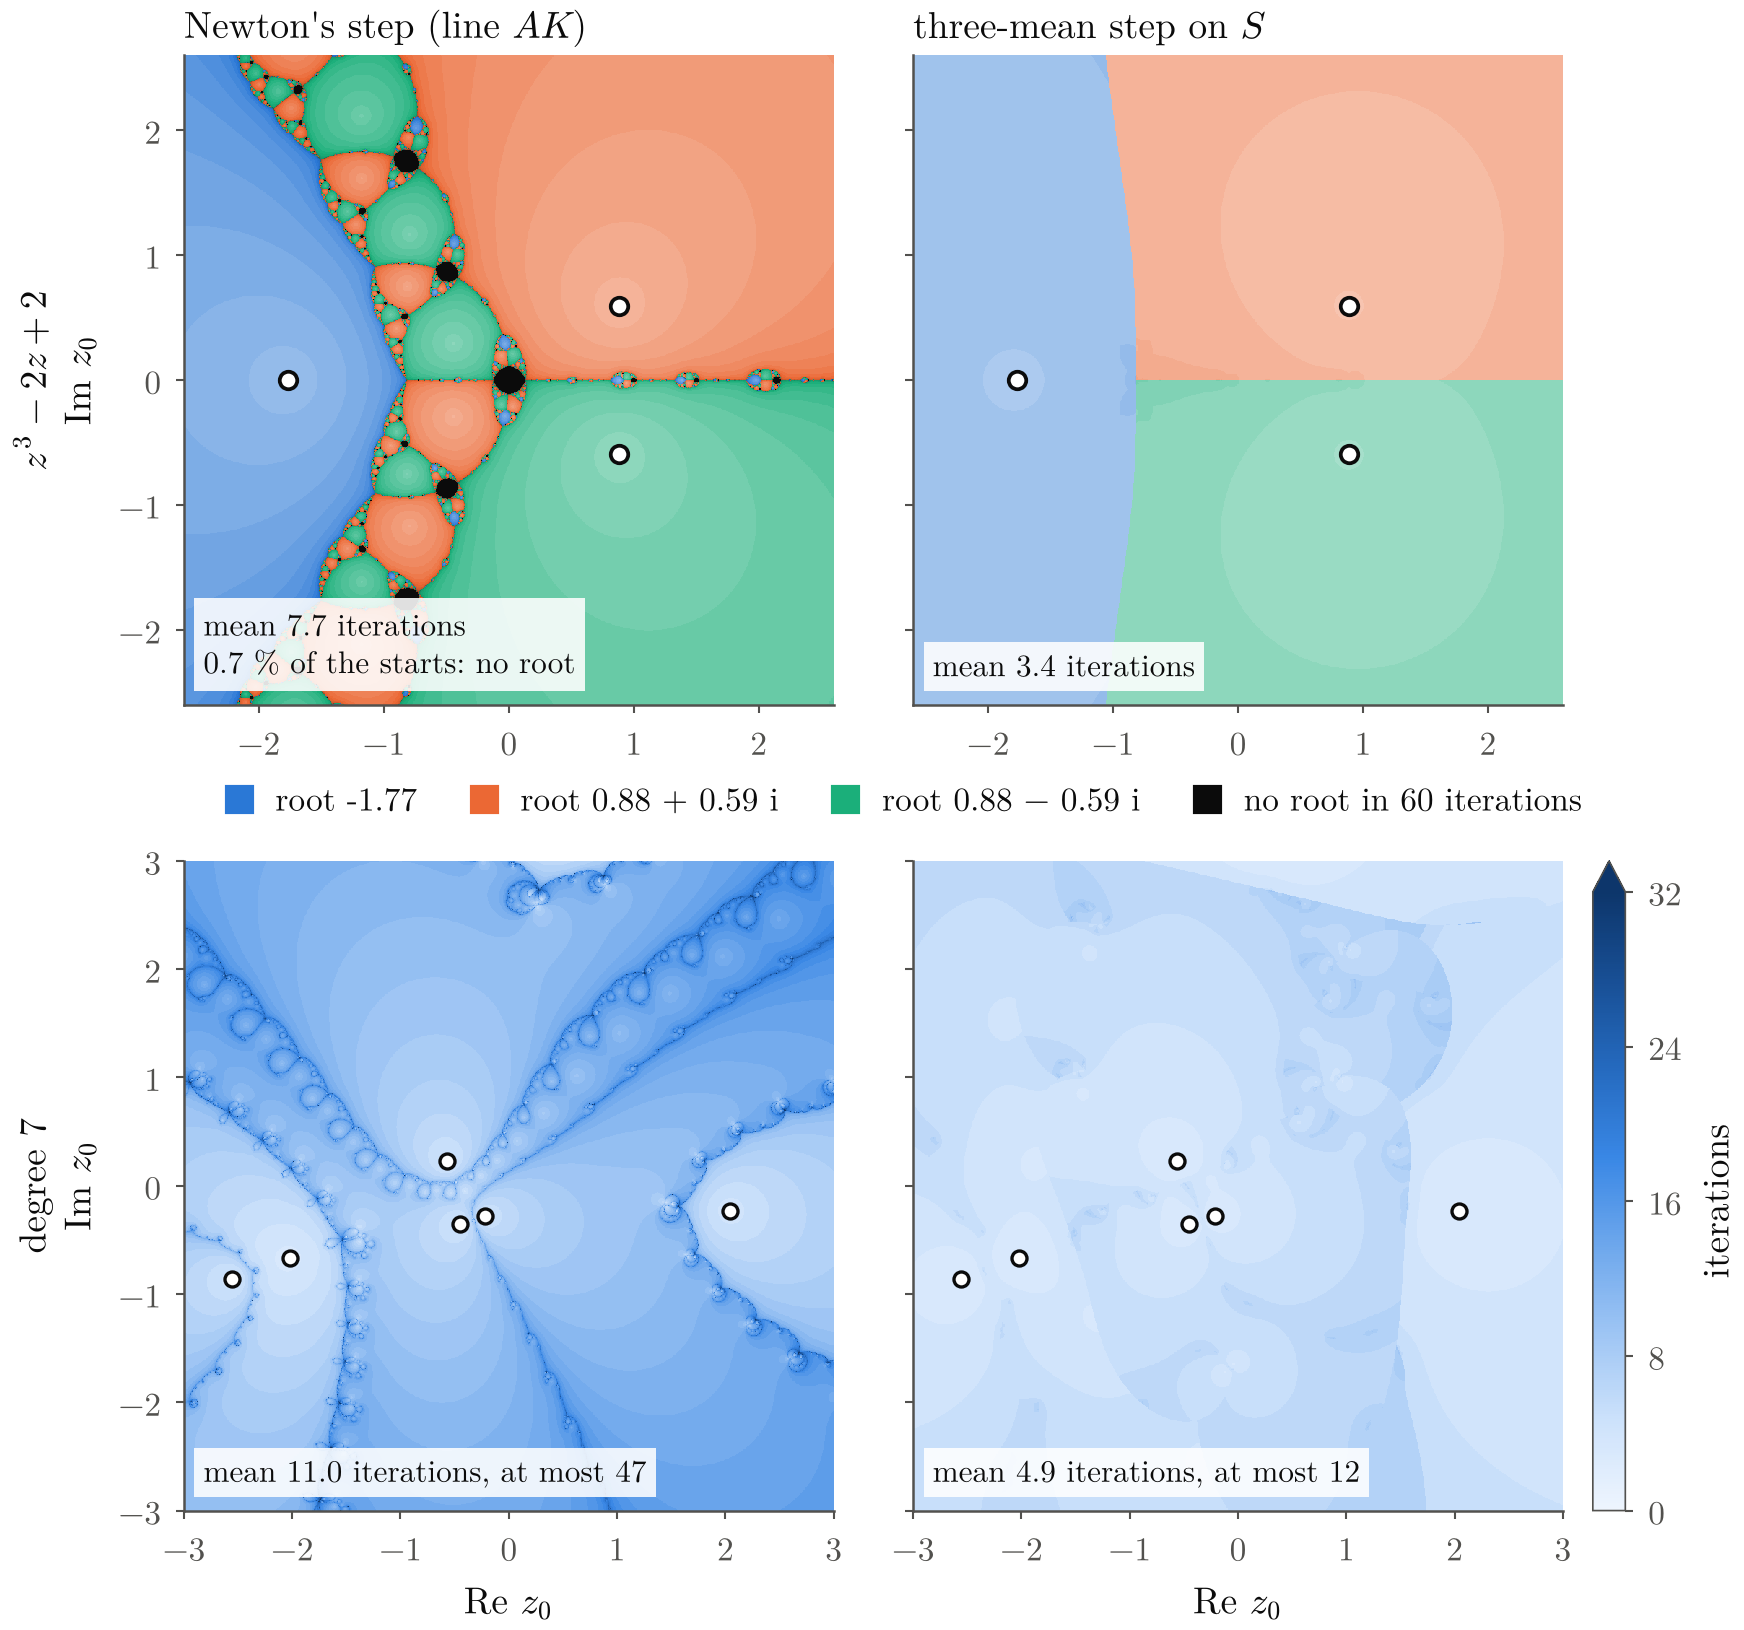
\includegraphics[width=\textwidth]{fig_onepoint.png}
\caption{The step for one root at a time, seen from every starting point $z_0$ of a window (900 by 900
points; white dots: the roots). Left: Newton's step, that is, the line $AK$. Right: the three-mean
step~\eqref{eq:g2} on $S$ itself, the one that announces the neighbours in a sweep. Top, $z^3-2z+2$:
the colour is the root reached, darker when more iterations are needed; Newton's step has the
attracting cycle $0\to1\to0$ and $0.7\,\%$ of the window never reaches a root (black). Bottom, a
polynomial of degree 7 with complex Gaussian roots: number of iterations. In both windows the
three-mean step reached a root from every point, in 3.4 and 4.9 iterations on average (Newton: 7.7
and 11.0). Two polynomials and two windows: an illustration, not a statement of global convergence;
the straight edges on the right are the branch cuts of the square roots.}\label{fig:onepoint}
\end{figure}

\section{Local order}\label{sec:order}
Let $e_k=z_k-\zeta_k$, $\eta_l=y_l-\zeta_l$, $\varepsilon=\max|e_k|$, $\eta=\max|\eta_l|$, and
\[
 \delta_1=\sum_{l\ne k}\Bigl(\frac1{z_k-\zeta_l}-\frac1{z_k-y_l}\Bigr),\qquad
 \delta_2=\sum_{l\ne k}\Bigl(\frac1{(z_k-\zeta_l)^2}-\frac1{(z_k-y_l)^2}\Bigr),
\]
both $O(\eta)$ when the roots are simple and the points close to them.

\begin{theorem}\label{thm:order}
Let $q$ be analytic near $1$ with $q(1)=1$, $q'(1)=\frac12$, $q''(1)=2q_2$, and let $p>1$. With
$x=\delta_1e_k$ and $v=\delta_2e_k^2$, the step~\eqref{eq:step} satisfies
\begin{equation}\label{eq:err}
 \frac{e_k^+}{e_k}=\frac v2+\Bigl(\frac12+\frac{4p\,q_2}{p-1}\Bigr)x^2+O\bigl(|x|^3+|xv|+|v|^2\bigr),
 \qquad\text{while for }q=1:\quad \frac{e_k^+}{e_k}=\frac{x}{1+x}.
\end{equation}
\end{theorem}
\begin{proof}
Since $S'/S=\sum_l1/(w-\zeta_l)$ and $(S'^2-SS'')/S^2=\sum_l1/(w-\zeta_l)^2$, \eqref{eq:AB} gives
$A_k=(1+x)/e_k$ and $B_k=(1+v)/e_k^2$. Hence
$t_k-1=\dfrac{p\,(v-2x-x^2)}{(p-1)(1+x)^2}$ and
$\dfrac{e_k^+}{e_k}=1-\dfrac{p}{(1+x)\bigl(1+(p-1)q(t_k)\bigr)}$. For $q=1$ this is $x/(1+x)$. Otherwise
$(p-1)q(t_k)=p-1+\frac{p(v-2x-x^2)}{2(1+x)^2}+\frac{p^2q_2}{p-1}\,\frac{(v-2x-x^2)^2}{(1+x)^4}+\dots$,
so that
\[
 (1+x)\bigl(1+(p-1)q(t_k)\bigr)=p\Bigl[1+\frac{x^2+v}{2(1+x)}+\frac{4p\,q_2}{p-1}x^2+\dots\Bigr],
\]
and~\eqref{eq:err} follows; the term in $x$ alone cancels.
\end{proof}

\begin{corollary}\label{cor:orders}
Near simple roots, with all errors of the same size:
\begin{center}\small
\begin{tabular}{llll}
\toprule
support on $F_k$ & announced positions & leading error & order\\
\midrule
$AK$ & none ($y=z$) & $\delta_1e_k^2$ & 3 (Ehrlich--Aberth)\\
$AK$ & step of order 3 on $S$ & $\delta_1e_k^2$, $\delta_1=O(\varepsilon^3)$ & 5\\
any $q$ with $q'(1)=\frac12$ & none & $\frac12\delta_2e_k^3$ & 4\\
any $q$ with $q'(1)=\frac12$ & step of order 3 on $S$ & $\frac12\delta_2e_k^3$, $\delta_2=O(\varepsilon^3)$ & 6\\
\bottomrule
\end{tabular}
\end{center}
The sweep of Definition~\ref{def:sweep} has order~6: the step of~\cite{g2} on $S$ has order~3, so
$\eta=O(\varepsilon^3)$.
\end{corollary}

\begin{remark}[Why the order 9 is lost]\label{rem:nine}
The line $AD$, the conic and the three means all satisfy $q'(1)=\frac12$, and the leading term
$\frac12\delta_2e_k^3$ of~\eqref{eq:err} contains neither the support nor the degree $p$. The reason is
that the deflated function is almost linear near its root: the cursor obeys
$t_k-1=O(\eta\varepsilon)$, so the support is read only through $q(1)$, $q'(1)$ and, in the next term,
$q''(1)$. In~\cite{v29} the three means reach order~9 because they follow the exact support of a
$p$-th root over a whole range of $t$; here that range has collapsed to the point $t=1$. The three
means do satisfy the hypotheses: their coefficients obey $2\mu+\gamma-\nu=1$, and this one identity
gives both $q_M(1)=1$ and $q_M'(1)=\frac12$. The only trace left of the support is
$q_2=-(p+1)/(12p)$, which turns the second coefficient of~\eqref{eq:err} into $(p-5)/(6(p-1))$. In multiprecision the first errors of the line $AD$, the
conic and the three means agree to four digits (Section~\ref{sec:evidence}).
\end{remark}

\begin{remark}[The line $AD$ exactly]\label{rem:ad}
For $q=(1+t)/2$ the expansion is exact: $(1+x)\bigl(1+(p-1)q(t_k)\bigr)=p\bigl(1+\frac{x^2+v}{2(1+x)}\bigr)$,
hence
\[
 \frac{e_k^+}{e_k}=\frac{x^2+v}{2+2x+x^2+v},\qquad
 \Bigl|\frac{e_k^+}{e_k}\Bigr|\le|x|^2+|v|\quad\text{as soon as }|x|\le\tfrac14,\ |v|\le\tfrac14 .
\]
The degree $p$ has disappeared. For a general support $q=1+\frac{t-1}2+r$ the denominator is
$p\bigl(1+\frac{x^2+v}{2(1+x)}\bigr)+(p-1)(1+x)\,r$: the support enters through the remainder $r$ only.
\end{remark}

\begin{figure}[!htbp]\centering
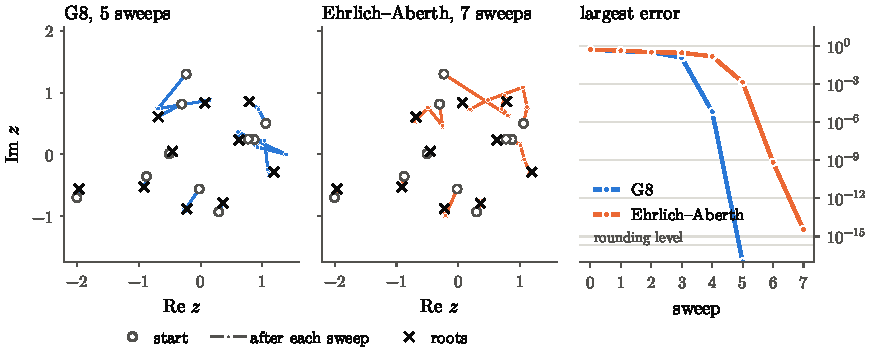
\includegraphics[width=\textwidth]{fig_paths.pdf}
\caption{One polynomial of degree 10 with complex Gaussian coefficients, from the start of
Section~\ref{sec:start}: the points after each sweep of G8 and of the Ehrlich--Aberth iteration, and
the largest distance from a point to a root. Most sweeps are spent approaching; the order shows in
the last two. This example needs 5 and 7 sweeps; the averages at degree 10 are 3.35 and 4.96
(Table~\ref{tab:random}).}\label{fig:paths}
\end{figure}

\section{One certificate}\label{sec:cert}
Let $z_1,\dots,z_m$ be distinct and $W_k=S(z_k)\big/\bigl(c\prod_{l\ne k}(z_k-z_l)\bigr)$: the
value at $z_k$ of the deflated function of Definition~\ref{def:defl} (with $y=z$), divided by $c$.

\begin{theorem}[Smith~\cite{smith}]\label{thm:smith}
Every root of $S$ lies in $\bigcup_kD(z_k,m|W_k|)$, and a connected component of this union made of
$q$ discs contains exactly $q$ roots.
\end{theorem}
\begin{proof}
The polynomial $\prod_l(w-z_l)+\sum_kW_k\prod_{l\ne k}(w-z_l)$ is monic of degree $m$ and equals $S/c$
at the $m$ points $z_k$, hence everywhere:
\begin{equation}\label{eq:pf}
\frac{S(w)}{c}=\prod_l(w-z_l)\Bigl(1+\sum_k\frac{W_k}{w-z_k}\Bigr)\qquad(w\ne z_1,\dots,z_m).
\end{equation}
It is the characteristic polynomial of $M=\operatorname{diag}(z_k)-W\mathbf 1^{\!\top}$, whose row $k$
has centre $z_k-W_k$ and off-diagonal sum $(m-1)|W_k|$. Gershgorin's theorems~\cite{gersh} apply.
(The first half also follows from~\eqref{eq:pf}: at a root that is not a node,
$1\le\sum_k|W_k|/|w-z_k|$, so one term is at least $1/m$.)
\end{proof}
The second half rests on a continuity argument. The count used by the algorithm is obtained in
another way, which needs Banach's fixed-point theorem only.

\begin{theorem}[Fixed-point certificate]\label{thm:fp}
Let $\rho\ge0$ with $\rho<|z_k-z_l|$ for every $l\ne k$, and
\[
\delta_l=|z_k-z_l|-\rho,\qquad\sigma=\sum_{l\ne k}\frac{|W_l|}{\delta_l},\qquad
\tau=\sum_{l\ne k}\frac{|W_l|}{\delta_l^2}.
\]
If $\sigma<1$, $|W_k|\le\rho(1-\sigma)$ and $|W_k|\tau<(1-\sigma)^2$, the closed disc $D(z_k,\rho)$
contains exactly one root of $S$.
\end{theorem}
\begin{proof}
Let $T(w)=\sum_{l\ne k}W_l/(w-z_l)$ and $\Phi_k(w)=z_k-W_k/(1+T(w))$. On the disc, $|w-z_l|\ge\delta_l$,
so $|T|\le\sigma$ and $|1+T|\ge1-\sigma>0$. By~\eqref{eq:pf}, for $w\ne z_k$ in the disc, $S(w)=0$ if
and only if $1+W_k/(w-z_k)+T(w)=0$, that is, $\Phi_k(w)=w$; and $S(z_k)=0$ if and only if $W_k=0$,
that is, $\Phi_k(z_k)=z_k$. So the roots of $S$ in the disc are the fixed points of $\Phi_k$. The disc
is mapped into itself: $|\Phi_k(w)-z_k|\le|W_k|/(1-\sigma)\le\rho$. Since
$\bigl|\frac1{w-z_l}-\frac1{w'-z_l}\bigr|\le|w-w'|/\delta_l^2$,
\[
|\Phi_k(w)-\Phi_k(w')|=\frac{|W_k|\,|T(w)-T(w')|}{|1+T(w)|\,|1+T(w')|}\le\frac{|W_k|\tau}{(1-\sigma)^2}\,|w-w'|,
\]
a contraction: one fixed point exactly.
\end{proof}
\begin{corollary}\label{cor:fp}
(i) If every $k$ satisfies Theorem~\ref{thm:fp} with a radius $\rho_k$ and the discs $D(z_k,\rho_k)$
are pairwise disjoint, $S$ has exactly one root in each disc and no other root.\\
(ii) Let $w_l\ge|W_l|$ for every $l$, $\rho=2w_k$, and let $\sigma,\tau$ be computed with the $w_l$.
If $\sigma<\frac12$ and $w_k\tau<\frac14$, Theorem~\ref{thm:fp} applies to $D(z_k,2w_k)$, and this disc
is disjoint from every $D(z_l,2w_l)$, $l\ne k$.
\end{corollary}
\begin{proof}
(i) The $m$ roots found are distinct and $S$ has at most $m$ roots. (ii) $1-\sigma>\frac12$ gives
$|W_k|\le w_k\le\rho(1-\sigma)$ and $|W_k|\tau<\frac14<(1-\sigma)^2$; each term of $\sigma$ is below
$\frac12$, so $2w_l<|z_k-z_l|-2w_k$.
\end{proof}
The code uses (ii), then (i). It replaces each gap $|z_k-z_l|-2w_k$ by a positive lower bound
(the computed distance, lowered): the sums only increase, so the test remains sufficient. Since
version 0.2.0 the test is made with the bounds $w_k(1+2^{-10})$ while the disc returned is
$D(z_k,2w_k)$: a returned disc may be enlarged by $2^{-10}$ of its radius (rounding of its centre to a
double, decimal printing) and still contain exactly one root. The point $\Phi_k(z_k)$ is the corrected point of
B\"orsch-Supan's iteration, and discs containing exactly one root were obtained by him from the same
Lagrange form~\cite{bs}; see also~\cite{bh}. No novelty is claimed for Theorem~\ref{thm:fp}; the constants
have not been compared with those of these papers. This version was chosen because its proof could be
formalised (Section~\ref{sec:evidence}). The hypothesis of the Gershgorin statement used in
revision~3 ($D(z_k,2|W_k|)$ disjoint from every $D(z_j,(2m-2)|W_j|)$) implies $\sigma<\frac12$: the
new test asks for less separation, and it adds the condition on $\tau$.

\begin{proposition}[Real roots]\label{prop:real}
Let $S$ be real, let discs $D_1,\dots,D_m$ contain all the roots of $S$, and let $D_k$ contain exactly
one root $\zeta$. Let $D$ be a disc centred on the real axis that contains $D_k$. If $D$ meets no
$D_j$, $j\ne k$, then $\zeta$ is real and is the only root of $S$ in $D$. If $D_k$ does not meet the
real axis, $\zeta$ is not real.
\end{proposition}
\begin{proof}
$D$ is its own mirror image, so $\overline\zeta$ is a root in $D$; every root in $D$ lies in some
$D_j$, hence in $D_k$, which contains one root only.
\end{proof}
The programs take $D=D(\operatorname{Re}z_k,\ \rho_k+|\operatorname{Im}z_k|)$ and return this disc for
a root flagged real. Revisions 1 to 6 tested the mirror image of $D_k$ only, which proves that the
root is real but not that the real disc returned is free of other roots; the test is now the one
stated. The discs are those of Corollary~\ref{cor:fp} when every $k$ passes, Smith's discs otherwise.

\begin{figure}[!htbp]\centering
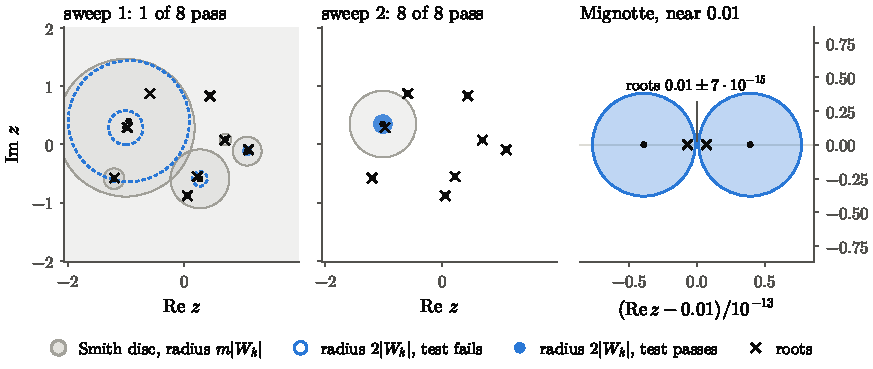
\includegraphics[width=\textwidth]{fig_discs.pdf}
\caption{The certificate on examples. Left and centre: a polynomial of degree 8 after the first and
the second sweep. After one sweep the largest Smith disc has radius 4.2 and covers the picture; one
disc $D(z_k,2|W_k|)$ passes the test of Corollary~\ref{cor:fp}\,(ii), although seven of them already
contain exactly one root: the test is sufficient, not necessary. After two sweeps the eight discs
pass; the largest has radius 0.14, inside its Smith disc of radius 0.57, and the seven others are too small to
be seen. Right: the two real roots of
Mignotte's polynomial $z^{12}-2(100z-1)^2$, $1.4\cdot10^{-14}$ apart, each in its disc of radius
$3.8\cdot10^{-14}$; the discs are disjoint, by $2.5\cdot10^{-15}$.}\label{fig:discs}
\end{figure}

\textbf{Arithmetic.} The certificate needs upper bounds of $|S(z_k)|$.
\begin{itemize}
\item \emph{First certificate.} $S(z_k)$ is computed in double precision; the bound is the computed
 modulus plus $4(m+1)\,2^{-52}\sum_j|c_j||z_k|^j$, a standard a priori bound for Horner's
 rule~\cite{higham}, which also covers the rounding of the coefficients (with an absolute term for
 underflow in the crate, Section~\ref{sec:rust}).
\item \emph{Values beyond double precision.} In the Python prototype the points are rounded to 53
 significant bits of their modulus; they are then Gaussian dyadic numbers and $S(z_k)$, $S'(z_k)$,
 $S''(z_k)$ are computed exactly with integers by Horner's rule ($O(m^2)$ integer operations for the
 $m$ points). The crate, since version 0.3.0, evaluates them in fixed point with a rigorous bound of
 the rounding (a ball, Section~\ref{sec:rust}), with as many bits as $|S(z_k)|$ needs to be known to
 the relative precision asked for; a value that cannot be told from zero is computed exactly.
\item The product $\prod_{l\ne k}|z_k-z_l|$ is computed in floating point with a relative margin
 $(8m+64)\,2^{-52}$; the sums $\sigma$ and $\tau$ with a margin $(2m+16)\,2^{-52}$, the distances
 being lowered by $8\cdot2^{-52}$.
\end{itemize}
\textbf{The certificate continues the iteration.} A disc $D(z_k,2w_k)$ is \emph{fine} if it passes
Corollary~\ref{cor:fp}\,(ii), its radius is at most $\mathrm{tol}\cdot|z_k|$ (default $10^{-10}$)
and, for real $S$, Proposition~\ref{prop:real} decides whether its root is real; or if it has
reached the floating-point grid. If some disc is not fine, the sweep of Definition~\ref{def:sweep} is
applied again to the points concerned, with the values of $S,S',S''$ known beyond double precision,
and the certificate is recomputed. This is the same iteration with better data, not another method:
the sums of~\eqref{eq:AB} are well-conditioned, only the values of $S$ near its roots are not.

\section{The start: dominant binomials}\label{sec:start}
Most sweeps are spent before the points are near the roots: on random polynomials started from one
circle, once every point is within a tenth of the smallest gap between roots, one sweep is enough,
and 3 to 8 sweeps come before (script \texttt{where.py}). The order of the iteration plays no part
there; the starting points do. The note~\cite{g7} started on one circle around the centroid, which
uses the pair of coefficients $(a_0,a_m)$ of the polynomial recentred. The following start reads all
the scales.

Write $S(z)=\sum_ja_jz^j$ and take the upper convex hull of the points $(j,\log|a_j|)$ (the Newton
polygon). An edge from $i$ to $k$ is a binomial $a_iz^i+a_kz^k$ that dominates the other terms, or
nearly so, on the circle $|z|=|a_i/a_k|^{1/K}$, $K=k-i$: this is the binomial of the lemma
of~\cite{g3}, here for every scale at once, and it announces $K$ roots of that modulus.
\begin{enumerate}
\item \emph{Groups.} An edge with $K=1$ is called soft if the other terms exceed twice the two terms
 of its binomial on its circle. A run of consecutive soft edges is merged into one group; every other
 edge is a group by itself.
\item \emph{A group $(i,k)$ is a shifted power.} With $q(z)=a_i+a_{i+1}z+\dots+a_kz^{K}$, its roots
 have centroid $g=-a_{k-1}/(Ka_k)$, and the points are $g+w^{1/K}$, the $K$ values of the $K$-th root
 of $w=-q(g)/a_k$, at their true angles (the angle section of~\cite{c5}). For $K=1$ the point is
 $-a_i/a_k$.
\item \emph{Real polynomials.} Each group with $K\ge2$ is turned by a tenth of its angular spacing,
 so that the start is not symmetric (Section~\ref{sec:trap}).
\end{enumerate}
When the polygon has a single edge this is the circle of~\cite{g7} with the right angles. The cost is
$O(m)$ per edge. The circles are those of Bini's start~\cite{bini}; what is added is the centroid and
the angles of each group. With arbitrary angles on the circles of the polygon the gain disappears:
4.45 sweeps against 4.37 for the single circle at degree 10 (5.49 against 5.16 at degree 20), and
3.37 (4.39) with the angles (script \texttt{start\_angles.py}).

\begin{table}[H]\centering\small
\begin{tabular}{lrr@{\qquad}lrr}
\toprule
polynomial & one circle & binomials & polynomial & one circle & binomials\\
\midrule
roots $10^k$, $k<10$ & 23 & 3 & Chebyshev 30 & 14 & 7\\
roots $2^k$, $k<20$ & 23 & 3 & Mignotte, degree 12 & 16 & 9\\
coefficients from $10^{-8}$ to $10^{8}$ & 23 & 2 & $\exp$ truncated, degree 40 & 15 & 9\\
$(z^{10}-1)(z^{10}-10^{20})$ & 20 & 2 & $(z-3)^{12}-5$ & 2 & 5\\
Wilkinson 20 & $9+17$ & $12+5$ & Wilkinson 10 & 7 & 9\\
\bottomrule
\end{tabular}
\caption{Sweeps in double precision (for Wilkinson 20: plus exact-value sweeps). Of the 21 families of
the script, the new start needs fewer sweeps in 12 and more in 5: the single circle remains better when
all the roots are grouped away from the origin. On random polynomials see Table~\ref{tab:random}.}
\end{table}

\begin{figure}[!htbp]\centering
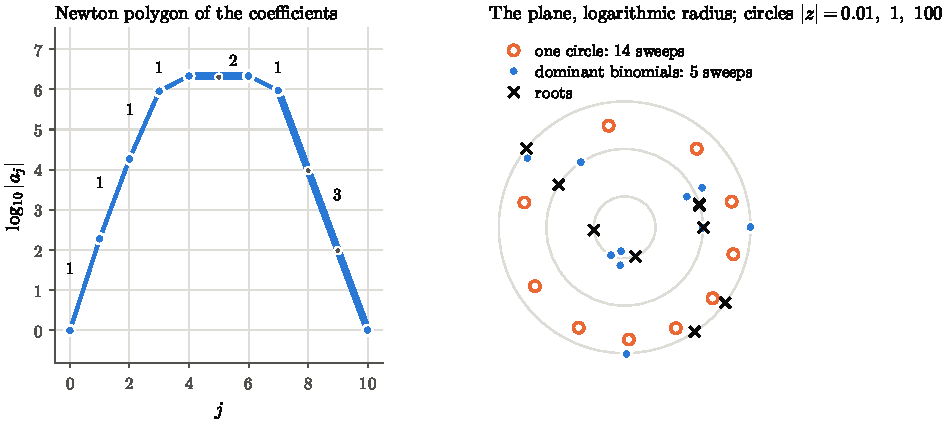
\includegraphics[width=\textwidth]{fig_start.pdf}
\caption{The start on a polynomial of degree 10 with roots at three scales (three near $|z|=0.01$,
four near 1, three near 100). Left: the points $(j,\log_{10}|a_j|)$ and the groups read on their upper
convex hull (numbers: roots announced by each group; thick: groups of two roots or more). Right: the roots, the start from the dominant binomials and the start from one circle;
from the first the sweeps of G8 need 5 sweeps, from the second 14.}\label{fig:start}
\end{figure}

\section{The algorithm}\label{sec:algo}
\begin{enumerate}
\item \emph{Square-free decomposition} $P=c\prod_kS_k^k$, exact~\cite{g5,g6}, skipped when the
 test modulo a prime of~\cite{g7} shows that $P$ is square-free.
\item For each factor $S$ of degree $m$: \emph{start} from the dominant binomials
 (Section~\ref{sec:start}).
\item \emph{Sweeps} of Definition~\ref{def:sweep} in double precision, until the residuals are at
 rounding level; at most $100+10m$.
\item \emph{Certificate} of Section~\ref{sec:cert}; while a disc is not fine, sweep with values known
 beyond double precision and certify again; at most $30+m$ certificates; the best certified state is
 kept. (The crate goes on at points with more bits when the tolerance or the separation of the roots
 asks for it, Section~\ref{sec:rust}.)

\item \emph{Output}: if every disc passes Corollary~\ref{cor:fp}, the $m$ discs $D(z_k,2w_k)$, one
 root in each. Otherwise (points that the floating-point grid cannot separate), for each component of
 the Smith discs, a disc and the number of roots it contains. In both cases the multiplicity $k$ and,
 for real $P$, the flag of Proposition~\ref{prop:real}.
\end{enumerate}

\begin{theorem}\label{thm:g8}
The algorithm stops. If the floating-point bounds (of $|S(z_k)|$, of the products, of the sums
$\sigma$ and $\tau$) are valid and the approximations of each factor are
distinct, every output disc with multiplicity $k$ and count $q$ contains exactly $q$ distinct roots
of $P$, each of multiplicity $k$; the counts weighted by the multiplicities add up to $\deg P$; a
root flagged real is real.
\end{theorem}
\begin{proof}
The loops are bounded. The rest is Corollary~\ref{cor:fp} or, in the second case of the output,
Theorem~\ref{thm:smith}; Proposition~\ref{prop:real}; and the square-free decomposition.
\end{proof}
Discs coming from two different factors $S_k$ are not compared with each other: they may overlap when
roots of different multiplicities are close; each statement remains true.
There is no branch to another method. What the theorem does not promise is small radii: if the
sweeps did not converge, the output would be the same list with large discs, possibly one disc
containing several roots. This did not happen in the tests of Section~\ref{sec:meas}: every final
count there came from Corollary~\ref{cor:fp}, the second case of the output was never used.

\section{A trap for real polynomials}\label{sec:trap}
\begin{proposition}\label{prop:trap}
Let $S$ be real with two real roots $x\pm d$, let two approximations be $x\pm iy$ and let the others
sit on the other roots. One Ehrlich--Aberth step sends $y=d\tan\theta$ to $d\tan3\theta$ and leaves
$x$ unchanged. More generally, for two approximations $x\pm w$ with any complex $w$, the step sends
$w$ to $w^+=w\,\dfrac{w^2+3d^2}{3w^2+d^2}$, and
\[
 \frac{w^+-d}{w^++d}=\Bigl(\frac{w-d}{w+d}\Bigr)^{3}.
\]
\end{proposition}
\begin{proof}
For the point $x+w$: $A=\frac1{w-d}+\frac1{w+d}-\frac1{2w}=\frac{3w^2+d^2}{2w\,(w^2-d^2)}$, so
$w-1/A=w\,\frac{w^2+3d^2}{3w^2+d^2}$; then $w^+\mp d=(w\mp d)^3/(3w^2+d^2)$. For $w=iy$ the
coordinate $(w-d)/(w+d)$ has modulus one and argument $\pi-2\theta$: the step is the cube on the
unit circle, the angle is tripled.
\end{proof}
In the coordinate $(w-d)/(w+d)$ the two roots are $0$ and $\infty$ and the trap is the unit circle,
which the cube maps to itself: this is the order three of Ehrlich--Aberth seen from the circle that
separates the two basins.
Tripling the angle never converges to $\theta=0$: in exact arithmetic the conjugate pair never
splits into the two real roots. The same holds for every sweep that commutes with complex
conjugation, in particular those of Section~\ref{sec:step} (off the branch cut of the square
roots): a conjugate pair stays conjugate. In double precision the asymmetric start makes the trap
unlikely. In the exact-value sweeps it can occur, because
rounded coefficients may turn two real roots into a conjugate pair; the pair is then released only by
the rounding of the sums. On Wilkinson's polynomial of degree 20 started from one circle this took 17
exact-value sweeps, against 1 to 10 in the other ill-conditioned cases. This escape is observed, not
proved.

\begin{remark}[The real axis, where the support matters]\label{rem:axis}
For a real polynomial, the Ehrlich--Aberth step sends real points to real points: approximations
that are all real can never reach a pair of complex roots. The square roots of the three means do
leave the axis (a negative cursor has an imaginary square root). With the start of
Section~\ref{sec:start}, which puts single-root groups on the real axis, one of the 400 real
polynomials of degree 5 of Section~\ref{sec:rust} is not solved by the line $AK$ (150 sweeps, two
clusters), and all are by the three means. This is the one place in this note where the support
changes the outcome and not only a count.
\end{remark}

\begin{figure}[!htbp]\centering
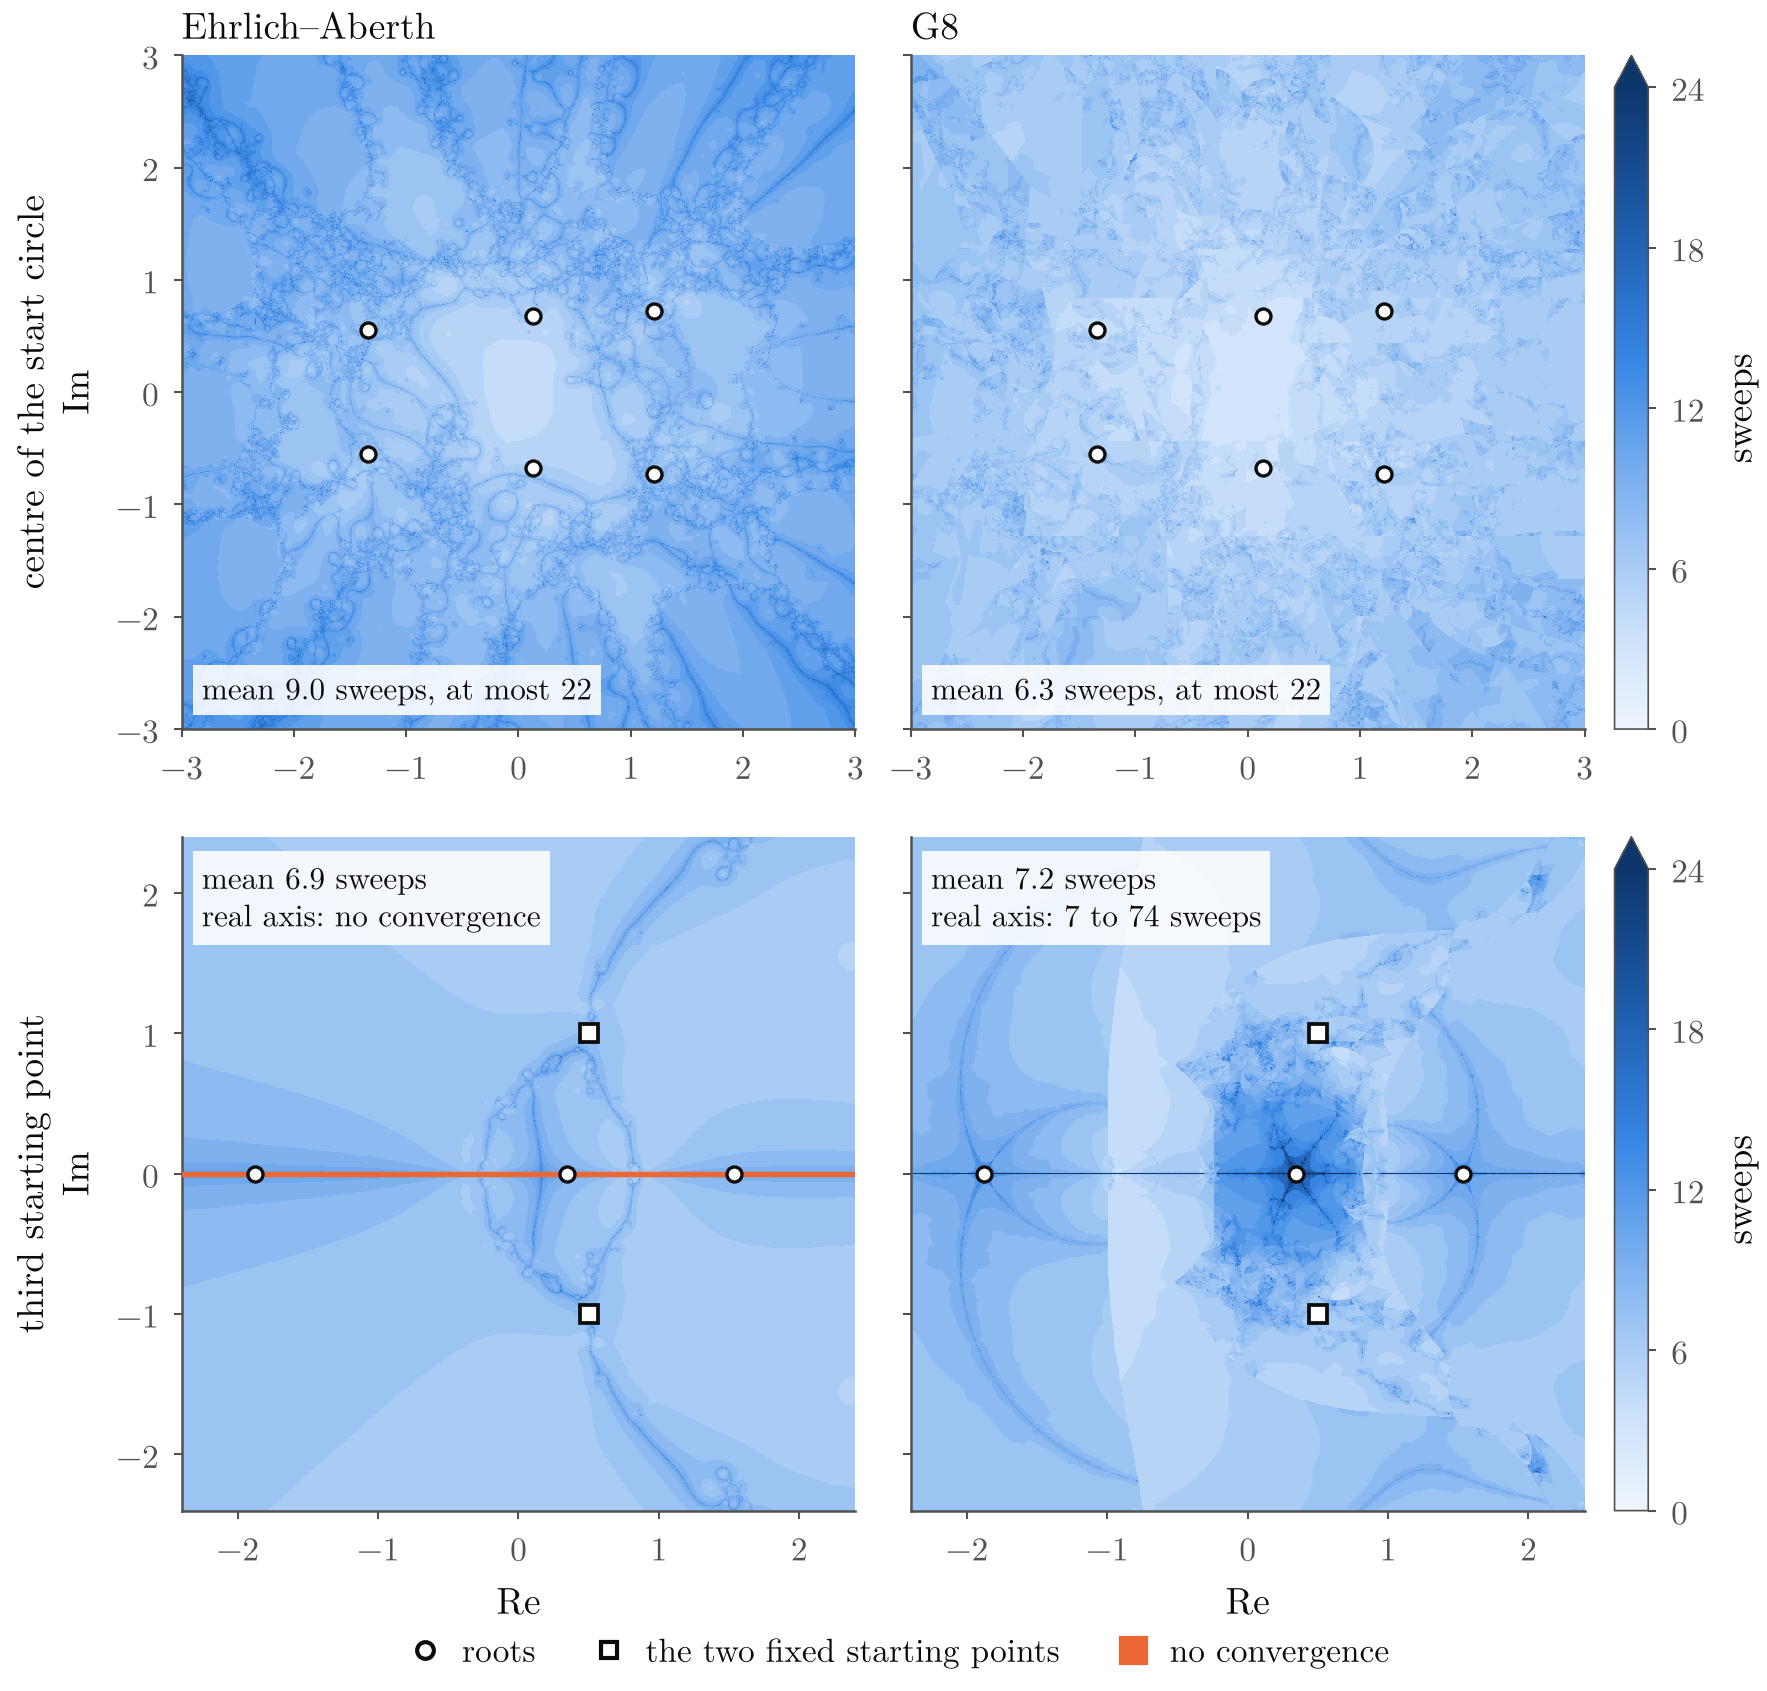
\includegraphics[width=\textwidth]{fig_sweeps.png}
\caption{Number of sweeps as a function of the start, on two slices of the space of starts (801 by
801 points). Top: a real polynomial of degree 6; the six points start on a circle of radius 1.3
whose centre moves over the window. Bottom: $z^3-3z+1$, which has three real roots; two points start
at $\frac12\pm i$ and the third one moves. When the third point is real the start is symmetric and
Proposition~\ref{prop:trap} applies: the Ehrlich--Aberth sweep stays symmetric (here its
floating-point operations keep the symmetry exactly) and none of the 801 points of the real axis
converges in 200 sweeps. The sweep of G8 loses the symmetry at the level of rounding in its first
sweeps and converges from every point of the axis, slowly (30 sweeps in the median, up to about 80;
these numbers depend on the rounding). Off the axis this cubic is not favourable to G8: 7.2 sweeps on
average against 6.9. The algorithm never starts on such an axis (Section~\ref{sec:start}).}\label{fig:sweeps}
\end{figure}

\section{Measurements}\label{sec:meas}
The numbers of this section come from the Python prototype (script \texttt{verify\_g8.py}); those of
Section~\ref{sec:rust} from the Rust crate (scripts \texttt{rust\_check.py}, \texttt{simple.py},
\texttt{underflow\_check.py} and \texttt{precise\_check.py}).

\textbf{Random polynomials} (Gaussian coefficients). All were certified: every root isolated in its own
disc, the result equal to that of \texttt{numpy.roots}; no exact-value sweep was needed. The median
over the polynomials of the largest relative radius goes from $2\cdot10^{-14}$ (degree 5) to
$6\cdot10^{-13}$ (degree 160).
\begin{table}[H]\centering\small\setlength{\tabcolsep}{4.5pt}
\begin{tabular}{lr@{\quad}rrr@{\qquad}rrr}
\toprule
 & & \multicolumn{3}{c}{complex coefficients} & \multicolumn{3}{c}{real coefficients}\\
degree & number & G8 & G8, one circle & E.--A. & G8 & G8, one circle & E.--A.\\
\midrule
5 & 400 & 2.54 (7) & 3.45 (8) & 3.91 (7) & 2.69 (8) & 4.04 (8) & 4.56 (149)\\
10 & 400 & 3.35 (8) & 4.32 (9) & 4.96 (11) & 3.51 (9) & 4.81 (12) & 5.35 (18)\\
20 & 300 & 4.29 (9) & 5.22 (14) & 6.26 (12) & 4.51 (11) & 5.85 (17) & 6.69 (14)\\
40 & 150 & 5.35 (11) & 6.09 (14) & 7.89 (13) & 5.72 (10) & 6.93 (21) & 8.42 (12)\\
80 & 40 & 6.72 (10) & 7.40 (10) & 9.03 (12) & 6.90 (12) & 7.92 (12) & 10.20 (13)\\
160 & 10 & 7.10 (9) & 8.40 (10) & 10.40 (15) & 8.00 (10) & 9.30 (15) & 11.00 (18)\\
\bottomrule
\end{tabular}
\caption{Mean number of sweeps in the Python prototype (maximum in brackets); 2600 polynomials in all
(the same number for each kind of coefficients). ``E.--A.'': Ehrlich--Aberth from the same start as
G8. G8 needs 26 to 41\,\% fewer sweeps than Ehrlich--Aberth, and 9 to 33\,\% fewer than from one
circle.}\label{tab:random}
\end{table}

\textbf{Which support.} 300 random polynomials of degree 10, 20, 40, half of them real; the roots are
compared with \texttt{numpy.roots}, without certificate.
\begin{table}[H]\centering\small
\begin{tabular}{llrrr}
\toprule
support on $F_k$ & announced by & all roots found & mean sweeps & maximum\\
\midrule
$AK$ (Ehrlich--Aberth) & nothing & 300 & 6.54 & 12\\
line $AD$ & nothing & 270 & 5.60 & 11\\
conic & nothing & 300 & 6.65 & 23\\
three means & nothing & 300 & 6.42 & 21\\
$AK$ & three means & 300 & 5.82 & 12\\
three means & line $AD$ (Halley) & 300 & 4.63 & 9\\
conic & conic & 300 & 4.38 & 10\\
three means & three means & 300 & 4.34 & 9\\
\bottomrule
\end{tabular}
\caption{The gain comes from using a second-order support twice. The three means and the conic are
equivalent within 1\,\%; the mean of the line $AD$ alone is over its 270 successes.}
\end{table}

\textbf{Hard families}, with exact coefficients. All roots were isolated and certified, and the real
roots proved real, in each of the 18 cases of the script; a selection:
\begin{table}[H]\centering\small
\begin{tabular}{lrrrl}
\toprule
polynomial & degree & float sweeps & certificates & largest relative radius\\
\midrule
$z^{50}-1$ & 50 & 2 & 1 & $4\cdot10^{-15}$\\
Wilkinson 15 & 15 & 8 & 2 & $3\cdot10^{-11}$\\
Wilkinson 20 & 20 & 12 & 6 & $2\cdot10^{-15}$\\
Wilkinson 30 & 30 & 12 & 9 & $5\cdot10^{-12}$\\
Chebyshev 30 & 30 & 7 & 2 & $9\cdot10^{-11}$\\
Mignotte $z^{12}-2(100z-1)^2$ & 12 & 9 & 6 & $4\cdot10^{-12}$\\
roots $10^k$, $k<10$ & 10 & 3 & 1 & $6\cdot10^{-14}$\\
five roots $10^{-4}$ apart & 7 & 7 & 7 & $3\cdot10^{-12}$\\
\bottomrule
\end{tabular}
\caption{One certificate means that the floating-point one sufficed. The two real roots of Mignotte's
polynomial, $1.4\cdot10^{-14}$ apart, are in two disjoint discs of radius $3.8\cdot10^{-14}$ and
proved real: the sweeps stop when the tolerance $10^{-10}$ is met and the real disc of
Proposition~\ref{prop:real} is clear, two certificates earlier than in revision~3, with larger discs.}
\end{table}

\textbf{Time of the Python prototype} (ms per polynomial, best of three runs, same polynomials).
\begin{table}[H]\centering\small
\begin{tabular}{lrrr@{\qquad}rrr}
\toprule
 & \multicolumn{3}{c}{complex coefficients} & \multicolumn{3}{c}{real coefficients}\\
degree & \texttt{numpy.roots} & G7 & G8 & \texttt{numpy.roots} & G7 & G8\\
\midrule
10 & 0.04 & 0.56 & 0.78 & 0.03 & 0.84 & 1.10\\
20 & 0.13 & 0.92 & 1.40 & 0.06 & 1.46 & 1.27\\
40 & 0.62 & 1.66 & 2.19 & 0.27 & 2.68 & 3.05\\
80 & 3.86 & 3.66 & 4.83 & 1.79 & 4.95 & 5.65\\
160 & 23.54 & 10.36 & 13.85 & 10.21 & 17.35 & 14.20\\
\bottomrule
\end{tabular}
\caption{In Python, G8 costs 0.8 to 1.5 times G7: fewer sweeps, each more expensive in NumPy, and the
start costs about the sweep it saves. The certified radii of G7 and G8 are the same on these
polynomials.}
\end{table}
On Wilkinson 20 the method of~\cite{g7} returned three discs and ``not complete'' after 3.1~s spent in
its rescue methods; G8 certifies the 20 roots in 6~ms. On Wilkinson 15 the largest radius falls from
$3\cdot10^{-3}$ to $2\cdot10^{-10}$.

\section{A Rust implementation}\label{sec:rust}
The crate \texttt{pandroots} (version 0.12.0 on crates.io, about 4500 lines without its tests, big
integers from \texttt{num-bigint} and, since 0.7.0, numbers of a fixed width in the inner loop of the
evaluations) implements the whole chain. It differs from the Python prototype in
four points.
\begin{itemize}
\item \emph{Gauss--Seidel order}: a point is used as soon as it has moved. This costs nothing in a
 compiled loop and removes 0.1 to 1.5 sweeps.
\item \emph{No overflow}: outside the unit disc $S'/S$ and $S''/S$ are computed through the reversed
 polynomial $w^mS(1/w)$. The first version evaluated $S$ directly and stopped converging from degree
 160, where $|S(z)|^2$ exceeds the range of double precision.
\item The exact coefficients (big integers) are built only if the certificate asks for values beyond
 double precision; the square-free test modulo a prime works on the doubles.
\item \emph{More digits than a double holds}: the same sweep and the same certificate continue at
 dyadic points of any size (below).
\end{itemize}
The double-precision part (start, sweeps, first certificate) is that of version 0.2.0: the source of
its sweep differs only by the new option of version 0.5.0, and the scaling of the variable chosen
since 0.3.0 is the identity for the polynomials of this section. Versions 0.6.0 to 0.12.0 do not
change it either: their additions are options, a second start that is used only when double precision
was not enough, and what happens before and after this stage.

\textbf{Validation} (version 0.12.0, the scripts of revision~7 run again). On the same files of
polynomials as \texttt{numpy.roots}: 2608 random polynomials of degree 5 to 320, all certified, every
root isolated and equal to that of \texttt{numpy.roots}, the number of roots proved real equal to the
number of real roots, the mean numbers of sweeps those of revision~7 within 0.01; the 17 hard families,
all certified (Wilkinson 20 in 0.6~ms, Wilkinson 30 in 2.0~ms; 1.2 and 5.5~ms with version 0.5.0); in
all of them the final count is that of Corollary~\ref{cor:fp}; exact multiplicities on 60 polynomials;
the 30 tests of the crate pass (19 integration tests, 9 unit tests, two documentation examples). The script \texttt{underflow\_check.py} of revision~7, against \texttt{mpmath} with 400 digits: of
195 polynomials at the edges of double precision, 189 certified sharply and 6 true but weak, none wrong
(0.2.0: 186 and 9); with the tolerance $10^{-20}$, 190 within the tolerance, 5 true but weak, none
wrong; its 31 polynomials with integer coefficients all certified within $10^{-30}$ and $10^{-80}$
(0.5 seconds each time for the 31, process start included; 0.7 and 1.3 seconds for 0.2.0 on the
machine of revision~7). The script reads the double precision output as doubles since this revision:
the crate prints the shortest decimal that reads back as the same double, and that decimal, read as an
exact number, is up to $10^{-16}$ of the centre away from the double, more than the radius of some discs
of version 0.12.0 ($3\cdot10^{-17}$ of the centre); read as exact decimals, six such discs were reported
wrong, and they contain their roots.

\textbf{Versions 0.2.0 and 0.3.0: defects found by a comparison with MPSolve.} An external check (a
harness comparing the crate with MPSolve~\cite{mpsolve}, run by the author with another assistant)
found that version 0.1.0 could return a wrong disc with \texttt{complete = true}: for
$2^{-1070}(z-1)(z-2)(z-3)$, whose coefficients are subnormal, a root was returned with radius zero.
The cause: the rounding bound of Horner's rule, $4(m+1)2^{-52}\sum_j|c_j||z|^j$, is relative, and says
nothing of an operation whose result underflows; when all the terms underflow the computed value and its
bound are both zero. Subnormal coefficients are not needed: $z^3-10^{-250}z$ fails in the same way near
its roots $\pm10^{-125}$. Of 195 polynomials at the edges of double precision (script
\texttt{underflow\_check.py}), version 0.1.0 gave 14 wrong answers and crashed on others. Version 0.2.0
changes four things.
\begin{itemize}
\item The variable is scaled by an exact power of two, $z=2^su$, and the coefficients by another one.
\item The bound becomes $\mu\bigl(\sum_j|c_j||z|^j+2^{-1020}\bigr)$, $\mu=4(m+1)2^{-52}$, which covers
 the operations that underflow (at most a few times $2^{-1074}$ each) and the scaled coefficients that
 became subnormal; outside the unit disc, where the point $1/z$ is itself rounded, $\mu$ is doubled
 (with $\mu$ alone the bound was not established for degrees above about 30); a leading coefficient
 that is no longer a normal number gives an infinite bound, hence values beyond double precision.
\item Distances and radii near the underflow threshold are computed after an exact scaling or
 refused; the output is sorted and merged without assuming finite numbers (no more crash).
\item The slack of Section~\ref{sec:cert} and the real disc of Proposition~\ref{prop:real}.
\end{itemize}
On the same 195 polynomials version 0.2.0 gives no wrong answer; 186 are certified sharply and 9 are
true but weak (\texttt{complete = false}, or one disc with several roots): polynomials whose
coefficients range from $10^{-300}$ to $10^{300}$, with roots that no double can hold. The same
comparison, on 462 polynomials up to degree 1024, then found three kinds of failure of 0.2.0 (7 cases of 462, none a
wrong answer), repaired in 0.3.0: the exponent $s$, chosen half-way between the extreme root moduli,
pushed most coefficients of a real polynomial of degree 1024 out of the range of doubles (a time-out);
it is now the $s$ for which the scaled coefficients spread over the fewest binary orders of magnitude,
$s=0$ for an ordinary polynomial. On Mignotte polynomials two points that had fallen on the same place
stayed together for ever (one disc of infinite radius, \texttt{complete = false}); one of them is now
moved aside. A polynomial of degree one kept a 53-bit centre; its root is now the quotient, rounded to
as many bits as asked for.

\textbf{Versions 0.6.0 to 0.12.0.} Seven changes around the sweep, none in its formula; the new step is
in Section~\ref{sec:cluster}.
\begin{itemize}
\item \emph{The root zero} (0.6.0). $P=z^kQ$ with $Q(0)\ne0$: the $k$ zero trailing coefficients are
 dropped, the root $0$ is returned with radius zero and multiplicity $k$, and only $Q$ is solved. The
 discs of $Q$ are kept if each is proved to stay away from $0$ (a count for $Q$ is then a count for $P$),
 otherwise $P$ is solved without deflation. A monomial costs nothing; before, a zero constant term sent
 the polynomial to Yun's algorithm.
\item \emph{Square-free decomposition} (0.6.0, 0.11.0). Yun's algorithm over the Gaussian rationals was
 replaced in 0.6.0 by pseudo-divisions over the Gaussian integers, and in 0.11.0 by gcds computed from
 their images modulo primes $p\equiv1\pmod 4$ (two images of a Gaussian integer per prime), put
 together by the Chinese remainder theorem and accepted only when they divide both polynomials exactly.
 The pseudo-remainder sequences kept the result right but not small: on 250 polynomials of degree about
 50 with multiple roots and 30-digit coefficients they met numbers of tens of thousands of bits and took
 87 seconds in all, against 0.05 with the modular gcd.
\item \emph{Numbers of a fixed width} (0.7.0). The Horner loop of the ball evaluation works on
 sign-magnitude numbers in buffers allocated once, and returns exactly the integers of the big-integer
 loop (exact products, shifts rounded towards minus infinity), so its error bound is unchanged. On
 Wilkinson 80 a profile gave 19\,\% of the time to the multiplications themselves and 75\,\% to
 allocation and bookkeeping.
\item \emph{The bits of each point} (0.8.0). In the sweeps with values beyond double precision each point
 starts from the number of bits its last evaluation needed, instead of 128 (on Wilkinson 80, 68\,\% of
 the evaluations were attempts with too few bits).
\item \emph{A scaled variable} (0.8.0, 0.10.1, 0.11.0). A double precision point $z$ far from the unit
 circle is evaluated through $T(t)=S(2^et)$ at $t=z/2^e$, $\frac12\le|t|<1$: the multiplier has the 53
 bits of the point, one or two limbs, instead of the bits of $1/z$. Horner's rule at $t$ loses up to $m$
 bits that the reversed polynomial does not lose when $z$ is just outside the unit circle, so this is used
 only when those bits are few against the bits of the evaluation (version 0.10.1: used for every point
 outside, it made a dense polynomial of degree 320 six times slower at 30 digits in versions 0.8.0 to
 0.10.0).
\item \emph{Coefficients beyond the range of doubles} (0.11.0). When the roots span more orders of
 magnitude than a double has, the coefficients do not fit in double precision next to one another; the
 points then start from the dominant binomials read on the exact coefficients and go straight to the
 sweeps with values beyond double precision.
\item \emph{A second start} (0.12.0). When double precision was not enough for a quarter of the points
 or more, the number of sweeps that follow depends on the start: 37 from the start of
 Section~\ref{sec:start} on Laguerre's polynomial of degree 150, 20 when each edge of the Newton polygon
 keeps its own binomial instead of being merged with its soft neighbours; on a Mandelbrot polynomial it
 is the reverse. Both sets of points are sampled (24 points at most) and the sweeps go on from the one
 whose median Smith radius is smaller, the second being taken only if it is $2^{16}$ times smaller.
\end{itemize}
The crate also has, since 0.8.0, the option \texttt{isolate} of Section~\ref{sec:cluster}, and its flag
\texttt{within\_tolerance} compares the radius with the modulus of the centre itself (up to 0.7.0 with a
power of two below it, which said no to discs within the tolerance by less than a factor of two).

\textbf{More digits than a double holds.} When the tolerance is below $10^{-12}$, or when double
precision could not separate or decide the roots, the sweep and the certificate continue at dyadic
points (module \texttt{precise}, functions \texttt{all\_roots\_precise} and
\texttt{all\_roots\_exact\_precise}; tolerances down to $10^{-280}$, points up to 4096 bits).
\begin{itemize}
\item \emph{Values.} The coefficients are scaled by a power of two and rounded to $F$ fractional bits;
 the point $x$ is $z$, or $1/z$ with the reversed polynomial, so that $|x|\le1$ and Horner's rule does
 not amplify the errors. With every product rounded downwards, the computed value $P$ satisfies
 $|P-2^FS(x)/2^E|\le A$, $A=1.01\,(m+1)\bigl(2.25+1.5\sum_j|c_j|/2^E\bigr)+1$ ($2^E$: the scale of the
 coefficients). $F$ is raised until $|P|\ge2^{r}A$, $r$ the relative precision asked for; the upper
 bound $|P|+A$ is the only number the certificate uses. Since 0.5.0, $S'$ and $S''$, which are not small
 near a root, are computed with fewer bits than $S$. Polynomials with few terms are evaluated term by
 term.
\item \emph{The step.} With $N=S/S'$, $\beta=SS''/S'^2$ at $z_k$, the sums
 $s_1=\sum_{l\ne k}(z_k-y_l)^{-1}$, $s_2=\sum_{l\ne k}(z_k-y_l)^{-2}$ of~\eqref{eq:AB}, $u=s_1N$ and
 $v=s_2N^2$, the step~\eqref{eq:step} with $p=m$ is
 \begin{equation}\label{eq:precise}
 \begin{gathered}
 (1-u)^2(t_k-1)=\frac{m\,(2u-u^2-\beta-v)}{m-1},\qquad \kappa=\frac{(m-1)\bigl(q(t_k)-1\bigr)}{m},\\
 z_k^+=z_k-\frac{N}{1+w},\qquad w=\kappa-u-u\kappa,
 \end{gathered}
 \end{equation}
 since $A_k=(1-u)/N$, $B_k=(1-\beta-v)/N^2$ and $1+(m-1)q=m(1+\kappa)$. Near the roots $w$ has the
 size of the error of the point, and the correction $Nw/(1+w)$ the size of its square. Since 0.4.0, by
 default, $N$ is a multiprecision quotient taken from the ball evaluation and only the correction is
 computed in double precision: a point with error $e$ goes to about $e^2\,2^{-50}$, the number of
 correct digits doubles at each sweep (up to 0.3.0 the whole step was in double precision, twelve to
 fifteen digits per sweep). With \texttt{Options::full\_order} (0.5.0) the announced positions, the
 sums and the support with its two square roots are computed in multiprecision as well, and each sweep
 keeps the order~6 of Corollary~\ref{cor:orders}, at the price of $m^2$ multiprecision divisions.
\item \emph{The certificate.} Corollary~\ref{cor:fp}\,(ii) with the ball bounds; the differences between
 points far apart are taken from their roundings to doubles (relative error below $2^{-28}$, a margin
 the test includes), closer ones are subtracted exactly. Only the points whose disc is not yet good
 enough are evaluated and moved; their number of bits doubles when they no longer move. A centre
 returned as a double has its radius enlarged by the exact distance to its rounding; the decimal output
 rounds the radius upwards within the slack $2^{-10}$ of Section~\ref{sec:cert}.
\end{itemize}
\emph{Checks of version 0.12.0} (script \texttt{precise\_check.py}, through \texttt{all\_roots\_exact\_precise}).
On 31 polynomials with integer coefficients (16 random of degree 5 to 40, Wilkinson 10 to 30, Chebyshev
10 to 30, two Mignotte polynomials, roots $10^{-20}$, $10^{-25}$ and $10^{-40}$ apart, roots $10^k$,
$z^{50}-1$, $z^2-2$), at the tolerances $10^{-30}$ and $10^{-80}$, by default and with
\texttt{full\_order}: 124 results of 124 are complete, every disc contains exactly one of the reference
roots computed independently by \texttt{mpmath} with 200 digits, and every radius is within the
tolerance (at most 0.90 of it). The flag \texttt{within\_tolerance} of the crate agrees in the 124 cases
(in revision~8 it said no once, on radii at 0.88 of the tolerance: it bounded $|z|$ from below by a power
of two; corrected in 0.8.0). The 31 polynomials take 22~ms in all at $10^{-30}$ and 30~ms at $10^{-80}$
(28 and 46~ms with 0.5.0). Larger polynomials, one call each, against references
computed in \texttt{mpmath} (Newton's method from \texttt{numpy.roots} for the dense ones,
\texttt{polyroots} for Wilkinson and Mignotte, exact for $z^{1000}-1$): all pass.
\begin{table}[H]\centering\small
\begin{tabular}{lrrr}
\toprule
polynomial & digits & default & \texttt{full\_order}\\
\midrule
dense, integer coefficients, degree 60 & 30 & 3.3 (1) & 3.4 (1)\\
 & 80 & 6.1 (2) & 12.6 (2)\\
 & 280 & 22.6 (4) & 29.4 (3)\\
dense, integer coefficients, degree 160 & 30 & 25.2 (1) & 24.4 (1)\\
 & 80 & 49.3 (2) & 66.6 (2)\\
 & 280 & 121 (4) & 151 (3)\\
dense, integer coefficients, degree 320 & 30 & 76.7 (1) & 68.8 (1)\\
 & 80 & 128 (2) & 239 (2)\\
 & 280 & 480 (4) & 704 (3)\\
$z^{1000}-1$ & 80 & 89.2 (2) & 957 (2)\\
 & 280 & 179 (4) & 1619 (3)\\
Wilkinson 30 & 80 & 2.6 (2) & 2.9 (2)\\
Mignotte $z^{12}-2(10^8z-1)^2$ & 30 & 0.5 (9) & 0.6 (5)\\
\bottomrule
\end{tabular}
\caption{Version 0.12.0, one call (milliseconds, best of three; in brackets the sweeps at points of more
than 53 bits), Apple M5, one thread, the machine in use by other programs. With version 0.5.0 in
revision~8: degree 60, 7.2, 15.7 and 33.2; degree 160, 32.9, 53.6 and 164; degree 320, 168, 231 and 668;
Wilkinson 30, 5.0; the Mignotte polynomial, 1.1 with 40 sweeps. At 280 digits the step of order six needs
three multiprecision sweeps instead of four, and is still slower: its $m^2$ multiprecision divisions cost
more than the sweep it saves, ten times more on $z^{1000}-1$, whose evaluation term by term is cheap. The
Mignotte pair, $1.4\cdot10^{-56}$ apart, is separated in 9 sweeps instead of 40: the step of
Section~\ref{sec:cluster}.}\label{tab:precise}
\end{table}

\textbf{Comparison with MPSolve.} The harness of the external check (not part of the crate) compares the
crate with MPSolve~3.2.3~\cite{mpsolve}, secular and standard algorithms, one thread, on 462 polynomials of
degree 1 to 1024 (314 random ones, integer and sparse ones, multiple roots, clusters, Mignotte
polynomials, roots of unity, Wilkinson, Chebyshev, monomials, extreme coefficients), and on 100 of them at
14, 30 and 80 digits. A case passes when the discs account for every root with its multiplicity, contain
the reference roots, and both the error and the radius are within the tolerance. It was run again, on
the same corpus and with the same scripts, for each version from 0.5.0 to 0.10.1, the version tested and
the previous one being measured in the same run with MPSolve.
\begin{table}[H]\centering\small
\begin{tabular}{lrrrr}
\toprule
 & \texttt{pandroots} 0.2.0 & 0.5.0 to 0.10.1 & MPSolve secular & MPSolve standard\\
\midrule
462 polynomials, 10 digits & 455 & 462 & 461 & 460\\
100 polynomials, 14 digits & & 100 & 99 & 97\\
100 polynomials, 30 digits & & 100 & 99 & 96\\
100 polynomials, 80 digits & & 100 & 99 & 81\\
\bottomrule
\end{tabular}
\caption{Passes. From 14 digits on, the crate is called through its \texttt{precise} functions, decimal
output included; the doubles interface cannot meet a tolerance below about $10^{-15}$. No disc of the
crate missed a reference root in any of these runs. MPSolve's misses are radii above the tolerance on
multiple roots, clusters and Mignotte pairs, one time-out, and covers that do not match the reference
roots with their multiplicities (Chebyshev 80 and 120, standard; $(z-1)^{10}(z+2)^{10}(z-i)^{10}$,
secular); each of them is passed by the other algorithm.}\label{tab:mpsolve}
\end{table}
\begin{table}[H]\centering\small
\begin{tabular}{lrr@{\qquad}lrr}
\toprule
 & 0.5.0 & 0.10.1 & family (10 digits) & 0.5.0 & 0.10.1\\
\midrule
462 polynomials, 10 digits & 2.95 & 4.06 & multiple roots (25) & 0.70 & 13.7\\
\quad crate faster on & 406 & 443 & Mignotte (9) & 0.15 & 1.54\\
100 polynomials, 14 digits & 0.61 & 2.04 & Chebyshev (5) & 0.70 & 1.45\\
100 polynomials, 30 digits & 0.63 & 2.03 & Wilkinson (5) & 0.33 & 0.84\\
100 polynomials, 80 digits & 1.03 & 3.14 & clusters of five roots (6) & 0.045 & 0.30\\
\quad crate faster on, at 80 digits & 64 & 80 & zero roots, monomials (8) & 0.005 & 0.45\\
\bottomrule
\end{tabular}
\caption{Geometric mean, over the cases both solve, of the time of MPSolve (its computation alone, the
faster of its two algorithms that pass) over the time of the crate (the whole call): above 1 the crate is
faster. Each column is its own run of the harness. The families of five to nine polynomials move by 30\,\%
from one run to the next on this machine. Version 0.12.0 was not run against MPSolve; its changes
(Laguerre polynomials, products with multiple roots and large coefficients, roots over hundreds of orders
of magnitude) touch families that this corpus does not have.}\label{tab:mpsolvetime}
\end{table}
MPSolve remains ahead on clusters of five roots (three to twelve times faster), on monomials and zero
roots (it removes them before its timed computation) and, by up to 30\,\%, on Wilkinson polynomials.

\textbf{The crate alone on 10\,000 polynomials} (version 0.12.0; script \texttt{gen10k.py} and example
\texttt{solveall}). Sixteen families: dense polynomials with five laws of coefficients, sparse ones,
prescribed rational roots, multiple roots, 1242 clusters of two to eight roots, Mignotte, roots in
arithmetic progression, orthogonal polynomials, powers, products, roots over many scales, the edges of
double precision, degrees up to 2000; 513\,018 roots in all. The figures are the solver's own (its flags
\texttt{complete} and \texttt{within\_tolerance}), one call per polynomial, one thread; the discs were
not checked independently on this corpus.
\begin{table}[H]\centering\small
\begin{tabular}{lrr}
\toprule
 & 0.10.1 & 0.12.0\\
\midrule
time for the 10\,000 polynomials & 111 s & about 15 s\\
complete & 9986 & 10\,000\\
every root in its own disc, within $10^{-10}$ & 9175 & 9189\\
\bottomrule
\end{tabular}
\caption{The 811 polynomials left out of the last line are clusters and Mignotte pairs that double
precision centres cannot separate: one disc with their number. Of the 111 seconds, 87 went to the
square-free decomposition of 250 products; the 14 incomplete answers were polynomials with roots over
more than 200 orders of magnitude. On the other 9986 polynomials the discs of 0.12.0 (multiplicities and
counts) are those of 0.10.1. Of the 15 seconds that remain, about 7 are double precision sweeps on sparse
and dense polynomials of degree 300 to 2000, and the rest sweeps of hundreds of bits on ill-conditioned
polynomials (15 to 40 of them each).}\label{tab:tenk}
\end{table}

\textbf{Time in double precision} (microseconds per polynomial, best of five runs, one thread).
\texttt{numpy.roots} calls compiled LAPACK through Python; the column ``LAPACK'' is the eigenvalue
routine alone, on a companion matrix built beforehand.
\begin{table}[H]\centering\small\setlength{\tabcolsep}{4.5pt}
\begin{tabular}{lrrrr@{\qquad}rrrr}
\toprule
 & \multicolumn{4}{c}{complex coefficients} & \multicolumn{4}{c}{real coefficients}\\
degree & sweeps & G8 Rust & \texttt{numpy.roots} & LAPACK & sweeps & G8 Rust & \texttt{numpy.roots} & LAPACK\\
\midrule
5 & 2.44 & 6.3 & 14.1 & 9.3 & 2.49 & 4.5 & 11.9 & 6.9\\
10 & 3.03 & 8.1 & 28.4 & 23.2 & 3.23 & 8.7 & 17.1 & 12.0\\
20 & 3.88 & 16.6 & 88.7 & 83.3 & 3.93 & 18.4 & 37.4 & 32.3\\
40 & 4.55 & 40.6 & 377 & 375 & 4.91 & 50.3 & 119 & 115\\
80 & 5.35 & 133 & 4062 & 4056 & 6.40 & 147 & 1068 & 1049\\
160 & 6.40 & 473 & 19310 & 19272 & 6.90 & 469 & 5511 & 5461\\
320 & 7.25 & 1795 & 109719 & 108577 & 8.75 & 1901 & 25477 & 25396\\
\bottomrule
\end{tabular}
\caption{Version 0.12.0, Apple M5, the machine in use by other programs. The same script with version
0.10.0, an hour earlier, gave ratios to \texttt{numpy.roots} from 2.4 to 58 (complex) and 2.0 to 12
(real), with times up to 1.7 times those of this table on some rows: the times move by 30\,\% or more
between runs. At real degrees 5 and 10 LAPACK alone takes about 1.4 to 1.5 times the time of G8.
The double-precision path is that of version 0.2.0 (Table~6 of revision~7, another machine).
G8 returns certified discs; LAPACK returns numbers.}\label{tab:time}
\end{table}
\textbf{Where the time goes, and what the support buys.} At degree 160 the sweeps take about two thirds
of the time, the certificate a quarter, the square-free test a tenth. The same code with other supports
(microseconds, mean sweeps in brackets, complex coefficients, best of 100 runs):
\begin{table}[H]\centering\small
\begin{tabular}{llrrr}
\toprule
support on $F_k$ & neighbours announced by & degree 20 & degree 80 & degree 320\\
\midrule
$AK$ (Ehrlich--Aberth) & nothing & 14.2 (5.51) & 117 (8.12) & 2085 (9.25)\\
$AK$ & their own step $AK$ & 14.7 (5.34) & 116 (7.67) & 2105 (9.25)\\
$AK$ & three means & 15.8 (4.65) & 152 (7.08) & 1920 (8.50)\\
three means & step $AK$ & 16.6 (4.21) & 184 (6.10) & 2590 (9.75)\\
three means & three means (G8) & 19.2 (3.88) & 143 (5.35) & 2085 (7.25)\\
\bottomrule
\end{tabular}
\caption{Fewer sweeps, about the same time: a sweep with the three means needs $S''$, a second sum and
four complex square roots per point. At degree 320 the two take the same time in this run (in the run of
revision~8 Ehrlich--Aberth was a quarter faster there, in that of revision~7 G8 was 8\,\% faster, and in
that of revision~3 Ehrlich--Aberth was ahead by about 15\,\% up to degree 20): the differences are of the
size of the noise of the machine. Announcing the neighbours by their own step $AK$ keeps the cost of
Ehrlich--Aberth and has local order 4~\cite{nourein}, but saves at most 8\,\% of the sweeps, because the
sweeps are spent far from the roots.}
\end{table}
For one root at a time nothing as simple as $AK$ can do better: an iteration without memory that
uses $S$ and $S'$ at one point has order at most two~\cite{traub}. The simultaneous setting escapes
this bound only because the neighbours bring information.

\section{The step of a cluster}\label{sec:cluster}
This section describes what versions 0.9.0 and 0.10.0 of the crate add to the sweep. It is used only for
points that share a tight cluster of roots; everywhere else the sweep is that of
Definition~\ref{def:sweep}. The certificate is computed after the points have moved, whatever moved
them: Theorem~\ref{thm:g8} is untouched.

\textbf{Why the sweep is slow near a cluster.} Theorem~\ref{thm:order} assumes simple roots with the
points close to them: the function deflated of the other points is then almost linear near its root,
which is where the order comes from. Let now $K$ roots lie within $\rho$ of a point $g$, and let the $K$
points meant for them be at a distance $d\gg\rho$ of $g$. Seen from there the cluster is one root of
multiplicity $K$, and each of the $K$ points is deflated of $K-1$ points that are as far from $g$ as it
is: $F_k$ is no longer close to linear, and the distance to the cluster is multiplied by a constant at
each sweep. In a multiprecision model of the sweep (script \texttt{cluster\_step.py}, the line $AD$ as
support) the factor is $\frac14$ for a pair, $0.40$ for three roots and $\frac47$ for five. This is the
linear convergence of simultaneous iterations at multiple roots, known for all of them.

\textbf{The cluster as a shifted power.} Seen from a distance $d\gg\rho$, the $K$ roots are those of a
function close to $(w-g)^K-a$, $|a|^{1/K}\approx\rho$: the function of the $K$-th root, for which the
rectangle with its exact support returns the root in one step~\cite{c5}. This is the model that the
start of Section~\ref{sec:start} applies once to each group of the Newton polygon; here it is applied
again, locally, whenever a cluster is seen.

\begin{proposition}\label{prop:cluster}
Let $f(w)=(w-g)^K-a$ with $K\ge2$, let $z$ be a point with $u=z-g\ne0$ and $f(z)\ne0$, and let
$A=f'/f$, $B=(f'^2-ff'')/f^2$ at $z$. Then
\begin{equation}\label{eq:cluster}
 t=\frac{KB-A^2}{(K-1)A^2}=\frac{a}{u^K},\qquad \frac{K}{A\,(1-t)}=u,
\end{equation}
and the $K$ roots of $f$ are the points $g+u\,\omega$, $\omega^K=t$.
\end{proposition}
\begin{proof}
$f=u^K-a$, $f'=Ku^{K-1}$, $f''=K(K-1)u^{K-2}$, so $A=Ku^{K-1}/(u^K-a)$ and
$B=Ku^{K-2}\bigl(u^K+(K-1)a\bigr)/(u^K-a)^2$. Then $KB-A^2=K^2(K-1)\,a\,u^{K-2}/(u^K-a)^2$, which
divided by $(K-1)A^2$ is $a/u^K$; $1-t=(u^K-a)/u^K$ gives $A(1-t)=K/u$; and
$(u\omega)^K-a=u^Kt-a=0$.
\end{proof}
The cursor $t$ of~\eqref{eq:cluster} is that of the step~\eqref{eq:step} with $p=K$: the step of
degree $K$, with the exact support of the $K$-th root, lands on the roots of the model, all of them at
once since the $K$ values of $t^{1/K}$ are available. For $K=2$ every quadratic is a shifted power and the
step is the solution of the quadratic. The $K$-th root is taken directly, as in the start of
Section~\ref{sec:start}, and not through the three means: these follow the exact support near $t=1$, and
here $t$ is near $0$.

\textbf{The step.} A \emph{tight} cluster is a connected component of $K\ge2$ overlapping Smith discs,
$K<m$, whose enclosing disc is at least 16 times smaller than its distance to the discs of the other
points. For such a component the polynomial is deflated of the points \emph{outside} it only: with one
point $z$ of the component,
\[
 A=\frac{S'(z)}{S(z)}-\sum_{l\notin C}\frac1{z-z_l},\qquad
 B=\frac{S'(z)^2-S(z)S''(z)}{S(z)^2}-\sum_{l\notin C}\frac1{(z-z_l)^2},
\]
then $t$ and $u$ by~\eqref{eq:cluster}, and the $K$ points of the component go to
$z-u+u\,t^{1/K}\omega^j$, each to the one nearest in angle. The step is used only if $|t|^{1/K}\le\frac14$
(the points are at least four times farther than the cluster is wide); otherwise the sweep does better.
It is used in the sweeps with values beyond double precision and in those at points of more bits, not in
the double precision stage.

\textbf{The cursor in multiprecision (0.10.0).} For a cluster seen from far, $t=(\rho/d)^K$ is tiny, and
$KB/A^2=1+(K-1)t$: the cursor is what is left of a number close to one. From $S'/S$ and $S''/S$ in double
precision it is lost below about $2^{-34}$; the centre $g=z-u$ is still found, but not the radius, and the
points were put on a circle of $2^{-30}$ of their distance and the step repeated. The ball evaluation of
Section~\ref{sec:rust} already returns $N=S/S'$ and $\beta=SS''/S'^2$ in multiprecision, and
\[
 A=\frac1N-s_1,\qquad B=\frac{1-\beta}{N^2}-s_2,\qquad t=\frac{K\,B/A^2-1}{K-1},
\]
with $s_1$, $s_2$ the two sums over the points outside. The evaluation is asked for
$K\log_2(d/r)+48$ bits of relative precision, $r$ being the radius aimed at: the spacing of doubles in the
doubles interface, the tolerance when roots closer than it need not be isolated, the grid of doubles in
the stage at double precision points. One evaluation then gives the radius of the cluster or shows that
it is below $r$. The double precision cursor is kept when it is above $2^{-24}$. After a step that
brings the points $q$ times closer, their next evaluation is asked $K\log_2(1/q)$ more bits at once, since
$S$ shrinks like the $K$-th power of the distance.

\textbf{Roots that doubles cannot tell apart (0.9.0).} With double precision centres, two roots closer
than the spacing of doubles are returned in one disc with their number: their discs overlap once the
centres are rounded. Up to version 0.8.0 they were first separated, with as many bits as it took (4096 for
$z^{40}-2(10^8z-1)^2$), then merged. The doubles interface now stops when the roots still together are in a
disc of relative radius below $2^{-54}$; the functions with centres of any precision separate as before.
The option \texttt{isolate} (0.8.0, \texttt{true} by default) extends this to the tolerance: with
\texttt{false} the solver stops as soon as every root is in a disc within the tolerance, alone or with the
roots it has not been told from. Either way the discs account for every root.

\begin{table}[H]\centering\small
\begin{tabular}{lrr}
\toprule
polynomial, 10 digits, doubles interface & without the step & with it\\
\midrule
five roots $10^{-30}$ apart & $25+17$ & $2+2$\\
five roots $10^{-12}$ apart & $24+0$ & $8+0$\\
Mignotte $z^{40}-2(10^8z-1)^2$ & $8+13$ & $0+1$\\
\bottomrule
\end{tabular}
\caption{Sweeps with values beyond double precision at double precision points, plus sweeps at points of
more bits, with the option \texttt{cluster} off and on (crate 0.10.0, both with the rule above for the
doubles interface). The five roots $10^{-12}$ apart are on a
line, not on a circle: the step brings the points to the cluster, and the sweep then needs eight passes to
separate them.}\label{tab:cluster}
\end{table}
In time, against version 0.8.0 on the same machine: $z^{40}-2(10^8z-1)^2$ from 13.0~ms to 0.32~ms, the
five roots $10^{-30}$ apart from 3.7~ms to 0.23~ms (Section~\ref{sec:rust}). What the step does not give:
it is exact for a shifted power only, and how close a cluster is to one is measured, not proved; a cluster
that contains all the points is left to the sweep; and on five roots the time left is that of the
evaluations at the five points, where $S$ is the fifth power of a small number and needs five times its
bits.

\section{Evidence and limits}\label{sec:evidence}
\textbf{Formalised in Lean~4} (Mathlib, toolchain v4.33.1; modules \texttt{SimultaneousRectangle},
\texttt{SmithDiscs} and \texttt{FixedPointCertificate}; 38 theorems, no \texttt{sorry}, the standard
axioms only; the same files as in revision~7, shipped in the \texttt{verification} folder of the crate
and not rebuilt since):
\begin{itemize}
\item Proposition~\ref{prop:step}: the cursor of the deflated function and the Ehrlich--Aberth case;
\item Theorem~\ref{thm:order}: the identities for $t_k-1$ and for $e_k^+/e_k$, the cancellation of the
 term in $x$ for every support with slope $\frac12$, the line $AD$ exactly with its bound
 (Remark~\ref{rem:ad}); for the three means, $q_M(1)=1$, $q_M'(1)=\frac12$ (as a derivative) and
 the coefficient $q_2$ (as an identity between the coefficients);
\item Theorem~\ref{thm:smith}, first half: the identity~\eqref{eq:pf} and the fact that every root
 lies in a disc $D(z_k,m|W_k|)$;
\item Theorem~\ref{thm:fp} (\texttt{existsUnique\_root}: the disc is mapped into itself, the Lipschitz
 bound, roots $=$ fixed points, existence and uniqueness by Mathlib's contraction theorem) and
 Corollary~\ref{cor:fp}\,(i) (\texttt{all\_roots\_certified});
\item Corollary~\ref{cor:fp}\,(ii) (\texttt{certificate\_of\_bounds}, \texttt{disjoint\_of\_bounds}) and
 the complete statement in the form the programs use (\texttt{all\_roots\_of\_computed}): let $S\ne0$
 have degree $m$ and leading coefficient $c$, let $w_l\ge|S(z_l)|/\bigl(|c|\prod_{j\ne l}|z_l-z_j|\bigr)$
 and $0<g_{kl}\le|z_k-z_l|-2w_k$; if $\sum_{l\ne k}w_l/g_{kl}<\frac12$ and
 $w_k\sum_{l\ne k}w_l/g_{kl}^2<\frac14$ for every $k$, then $S$ has exactly $m$ roots, one in each disc
 $D(z_k,2w_k)$ (the points are then distinct; this is proved, not assumed);
\item Proposition~\ref{prop:real}: in a general form (\texttt{real\_root\_of\_mirror}) and joined to the
 statement above in the form the programs test (\texttt{real\_disc\_of\_computed}: real coefficients,
 the same test, and $|\operatorname{Re}z_k-z_j|>2w_k+|\operatorname{Im}z_k|+2w_j$ for every $j\ne k$;
 then the root in $D(z_k,2w_k)$ is real and is the only root in the real disc returned);
 Proposition~\ref{prop:trap} in its general form.
\end{itemize}
For what the crate added from 0.6.0 to 0.10.0, five more files (31 theorems, no \texttt{sorry}, the
standard axioms; checked with Lean 4.35.0 and Mathlib v4.35.0, in the \texttt{verification} folder):
\begin{itemize}
\item \texttt{ZeroDeflation}: zero trailing coefficients give $P=X^kQ$; the roots of $X^kQ$ are $0$,
 $k$ times, and those of $Q$; the multiplicity of $0$ is $k$ when $Q(0)\ne0$; a disc with $|z|>r$ holds
 the same roots of $P$ as of $Q$;
\item \texttt{FixedWidth}: the floor of a negative quotient from the division of its magnitude, and the
 difference of two magnitudes computed modulo $2^{64n}$, with and without a borrow: the two identities
 behind the sign-magnitude arithmetic;
\item \texttt{ScaledVariable}: for $T(t)=S(ct)$, $T'=c\,S'$, $T''=c^2S''$ at the scaled point, the
 leading coefficient, the Newton term and the invariance of $SS''/S'^2$; a Smith disc lies in the disc
 that encloses its component;
\item \texttt{ClusterStep}: Proposition~\ref{prop:cluster};
\item \texttt{ClusterCursor}: $S'/S$ and its derivative from $N$ and $\beta$, the two forms of the
 cursor, its invariance under the scaling used.
\end{itemize}
So the chain from the inequalities tested by the programs to ``one root in each disc, no other root,
real where flagged'' is formal, at any precision of the points: the statement asks for upper bounds
$w_l$ and lower bounds $g_{kl}$, whatever arithmetic produced them. \emph{Not formalised:} the fact
that the numbers of the programs are such bounds (Horner's rounding bound and its underflow term, the
ball evaluation of the crate, the margins on the products, the distances and the sums); the second half
of Theorem~\ref{thm:smith} (a component of $q$ discs contains $q$ roots; Gershgorin's second theorem is
not in Mathlib), which the algorithm uses only for points that the grid cannot separate, never in the
tests; the expansion~\eqref{eq:err} for a general support beyond the cancellation identity; the
identity~\eqref{eq:precise}; the square-free test and Yun's algorithm (its gcds are checked by exact
division); how close a cluster is to a shifted power; the arithmetic of the crate on numbers of a fixed
width (tested against big integers), its choice between two starts, and the programs.

\textbf{Written proofs:} Proposition~\ref{prop:step}, Theorem~\ref{thm:order},
Theorem~\ref{thm:smith} (classical), Theorem~\ref{thm:fp}, Corollary~\ref{cor:fp},
Propositions~\ref{prop:real}, \ref{prop:trap}, \ref{prop:cluster}, Theorem~\ref{thm:g8}, the
identity~\eqref{eq:precise}.
\textbf{Checked numerically} (30 checks, all passed): the identities of
Section~\ref{sec:step} to 60 digits; the orders 3, 4, 5, 6 in multiprecision (observed 3.017, 4.003,
5.014, 6.007), the equality of the first errors for the three second-order supports (ratios
$1\pm2\cdot10^{-5}$) and the leading term $\frac12\delta_2e_k^3$; Smith's theorem and the fixed-point
certificate on 104 random states with errors from $10^{-9}$ to $0.5$ (776 discs pass, each with one
root; 29 of them are not isolated in Smith's sense; no isolated Smith disc fails); the final count is
that of Corollary~\ref{cor:fp} for the 2600 random polynomials and the 18 families; the tables above;
exact multiplicities on 43 polynomials; the two starts on 21 families. The Rust crate is validated
separately (Section~\ref{sec:rust}).

\textbf{Not new.} The Ehrlich--Aberth iteration; simultaneous iterations of Laguerre type~\cite{hpr};
raising their order to five and six by Newton's and Halley's corrections of the
neighbours~\cite{nourein,ppz}, and the same for the Hansen--Patrick family~\cite{hp,prp}, whose basic
order is four; Smith's discs; discs with exactly one root from the Lagrange form~\cite{bs,bh}; exact
residuals for the last digits; multiprecision with a precision raised as the iteration converges and
inclusion discs, as in MPSolve~\cite{mpsolve}; starting points on the circles of the Newton
polygon~\cite{bini}; the Gauss--Seidel order. The iteration of Definition~\ref{def:sweep} belongs to
this family. What is specific to this note: the derivation from the rectangle
(Proposition~\ref{prop:step}), the three-mean support in both places, the expansion that makes the
support disappear from the leading term (Theorem~\ref{thm:order}), the centroid and the angles of each
group of the start, the single path with exact-value sweeps, and the measurements. Restarting a
simultaneous iteration on a cluster from a shifted model of it is done in MPSolve~\cite{mpsolve}; what
Section~\ref{sec:cluster} adds is reading it as the step of degree $K$ of the same rectangle, on the
polynomial deflated of the points outside the cluster.

\textbf{Limits.}
\begin{itemize}
\item No theorem of global convergence: as for Ehrlich--Aberth, convergence from the start
 is observed, not proved. Theorem~\ref{thm:g8} guarantees the truth of the output, not its
 sharpness.
\item The three means do not beat the conic support (4.34 against 4.38 sweeps), and Halley's
 announcement is within 7\,\%. The order~9 of~\cite{v29} is lost for a structural reason
 (Remark~\ref{rem:nine}). In compiled code the three means do not beat Ehrlich--Aberth in time either:
 about the same time at every degree in the run of this revision (within the noise; a third more at
 degree 320 in the run of revision~8 and 8\,\% less in that of revision~7), for a quarter to a third
 fewer sweeps. Their one
 qualitative advantage observed is Remark~\ref{rem:axis}.
\item The start is better on average, not always: it loses on polynomials whose roots are grouped
 away from the origin (Section~\ref{sec:start}).
\item The symmetric trap of Section~\ref{sec:trap} is left by rounding; no escape is proved and none
 is built in.
\item The rounding bound of the first certificate, its underflow term, the ball evaluation and the
 margins on the products and the distances are not formalised; Lean proves the theorem that the
 certificate applies, not that the program applies it correctly. The guards near the underflow
 threshold are tested, not proved; polynomials whose roots span more than the range of a double get
 true but weak answers in the doubles interface.
\item The fixed-point certificate stops as soon as the tolerance is met: two very close roots get
 disjoint discs that may be much larger than their distance (Mignotte's polynomial above). A smaller
 \texttt{tol} gives smaller discs.
\item The step of a cluster is proved for a shifted power only; on a real cluster it is a proposal that
 the certificate judges afterwards. It closes on a cluster in one or two evaluations, but separating
 five roots, or certifying a disc around them, still takes evaluations with five times the bits of the
 distance: clusters of five roots remain three to twelve times slower than with MPSolve.
\item The choice between the two starts (0.12.0) is a measurement on a sample of points, with a margin
 set by trial on 10\,000 polynomials; it helps Laguerre polynomials and changes little elsewhere. The
 number of sweeps of hundreds of bits on ill-conditioned polynomials (15 to 40) is not explained by the
 local order; it is the price of the approach from the start, as in Section~\ref{sec:start}.
\item The Python prototype works in double precision only: roots that 53 bits cannot separate are
 reported together with their number. The crate goes on with more bits, up to 4096, in its functions with
 centres of any precision; its doubles interface, since 0.9.0, leaves together the roots that doubles
 cannot tell apart. A pair of roots closer than 4096 bits allow is reported as one disc with two roots (by
 default, $z^{40}-2(10^8z-1)^2$, whose pair is $1.4\cdot10^{-168}$ apart).
 The step of order six in multiprecision is not the default because it is not faster: its $m^2$
 multiprecision divisions per sweep cost about one evaluation of the polynomial at all the points, and
 it saves at most one. Outside the dense Horner loop (0.7.0) the big integers are those of
 \texttt{num-bigint}, and nothing runs in parallel.
\item Timings: one machine, one thread, variations of 20 to 30\,\% between runs; random
 polynomials are easy for every method. \texttt{numpy.roots} is a general eigenvalue solver applied to
 a companion matrix, not a specialised polynomial solver. The comparison with MPSolve uses one corpus
 and a harness outside the crate; its references are in part computed with MPSolve itself. The run on
 10\,000 polynomials reports the solver's own flags, without an independent check of its discs; three
 defects of the versions published on the way (a slowdown at large degree in 0.9.0 and 0.10.0, the slow
 square-free decomposition since 0.6.0, the incomplete answers on wide scales) were found by widening the
 corpus, after the comparison on 462 polynomials had passed.
\end{itemize}

\begin{thebibliography}{99}\small
\bibitem{aberth} O.~Aberth. Iteration methods for finding all zeros of a polynomial simultaneously.
 \emph{Math. Comp.} 27 (1973), 339--344.
\bibitem{bs} W.~B\"orsch-Supan. Residuenabsch\"atzung f\"ur Polynom-Nullstellen mittels
 Lagrange-Interpolation. \emph{Numer. Math.} 14 (1970), 287--296.
\bibitem{bh} D.~Braess, K.~P.~Hadeler. Simultaneous inclusion of the zeros of a polynomial.
 \emph{Numer. Math.} 21 (1973), 161--165.
\bibitem{bini} D.~A.~Bini. Numerical computation of polynomial zeros by means of Aberth's method.
 \emph{Numer. Algorithms} 13 (1996), 179--200.
\bibitem{mpsolve} D.~A.~Bini, L.~Robol. Solving secular and polynomial equations: a multiprecision
 algorithm. \emph{J. Comput. Appl. Math.} 272 (2014), 276--292.
\bibitem{v29} I.~Besevic. \emph{Geometric Root Calculators}, version V29, 2026.
\bibitem{c5} I.~Besevic. \emph{Complex Geometric Root Calculators}, version C5, 2026.
\bibitem{g2} I.~Besevic. \emph{Geometric Root Calculators for arbitrary polynomials: the anchored
 rectangle}, version G2, 2026.
\bibitem{g3} I.~Besevic. \emph{A globally convergent geometric calculator for every complex
 polynomial}, version G3, 2026.
\bibitem{g5} I.~Besevic. \emph{All real roots, with their multiplicities}, version G5, 2026.
\bibitem{g6} I.~Besevic. \emph{All the roots of a polynomial, with their multiplicities}, version G6,
 2026.
\bibitem{g7} I.~Besevic. \emph{Find, certify, count}, version G7, 2026.
\bibitem{ehrlich} L.~W.~Ehrlich. A modified Newton method for polynomials. \emph{Comm. ACM} 10 (1967),
 107--108.
\bibitem{gersh} S.~Gerschgorin. \"Uber die Abgrenzung der Eigenwerte einer Matrix. \emph{Izv. Akad.
 Nauk SSSR} 7 (1931), 749--754.
\bibitem{hp} E.~Hansen, M.~Patrick. A family of root finding methods. \emph{Numer. Math.} 27 (1977),
 257--269.
\bibitem{hpr} E.~Hansen, M.~Patrick, J.~Rusnak. Some modifications of Laguerre's method. \emph{BIT} 17
 (1977), 409--417.
\bibitem{higham} N.~J.~Higham. \emph{Accuracy and Stability of Numerical Algorithms}, 2nd ed. SIAM,
 2002.
\bibitem{nourein} A.-W.~M.~Nourein. An improvement on two iteration methods for simultaneous
 determination of the zeros of a polynomial. \emph{Int. J. Comput. Math.} 6 (1977), no.~3.
\bibitem{ppz} M.~S.~Petkovi\'c, L.~D.~Petkovi\'c, D.~\v{Z}ivkovi\'c. Laguerre-like methods for the
 simultaneous approximation of polynomial zeros. In \emph{Topics in Numerical Analysis}, Computing
 Supplementum 15, Springer, 2001.
\bibitem{prp} L.~D.~Petkovi\'c, L.~Ran\v{c}i\'c, M.~S.~Petkovi\'c. An efficient higher order family
 of root finders. \emph{J. Comput. Appl. Math.} (2008), 56--72.
\bibitem{smith} B.~T.~Smith. Error bounds for zeros of a polynomial based upon Gerschgorin's theorems.
 \emph{J. ACM} 17 (1970), 661--674.
\bibitem{traub} J.~F.~Traub. \emph{Iterative Methods for the Solution of Equations}. Prentice-Hall,
 1964.
\end{thebibliography}
\end{document}
